\documentclass[twoside,11pt]{article}
\usepackage{graphicx}
% \usepackage[draft]{graphicx}
\pagestyle{myheadings}

% -----------------------------------------------------------------------------
% ? Document identification - generic part
\newcommand{\stardoccategory}  {Starlink User Note}
\newcommand{\stardocinitials}  {SUN}
\newcommand{\stardocsource}    {sun\stardocnumber}
% -----------------------------------------------------------------------------
% ? Document identification - document specific part
% \newcommand{\stardocnumber}    {212.11 -- Draft}
\newcommand{\stardocnumber}    {212.12}
\newcommand{\stardocauthors}   {S.\,E.\,Rankin, M.\,J.\,Bly}
\newcommand{\stardocdate}      {21 July 2003}
\newcommand{\stardoctitle}     {Starlink Software CD--ROMs}
\newcommand{\stardocversion}   {Summer 2003}
\newcommand{\stardocmanual}    {User's Guide}
\newcommand{\stardocabstract}  {}

% ? End of document identification

% -----------------------------------------------------------------------------

\newcommand{\stardocname}{\stardocinitials /\stardocnumber}
\markboth{\stardocname}{\stardocname}
\setlength{\textwidth}{160mm}
\setlength{\textheight}{230mm}
\setlength{\topmargin}{-2mm}
\setlength{\oddsidemargin}{0mm}
\setlength{\evensidemargin}{0mm}
\setlength{\parindent}{0mm}
\setlength{\parskip}{\medskipamount}
\setlength{\unitlength}{1mm}

% -----------------------------------------------------------------------------
%  Hypertext definitions.
%  ======================
%  These are used by the LaTeX2HTML translator in conjunction with star2html.

%  Comment.sty: version 2..0, 19 June 1992
%  Selectively in/exclude pieces of text.
%
%  Author
%    Victor Eijkhout                                      <eijkhout@cs.utk.edu>
%    Department of Computer Science
%    University Tennessee at Knoxville
%    104 Ayres Hall
%    Knoxville, TN 37996
%    USA

%  Do not remove the %begin{latexonly} and %end{latexonly} lines (used by
%  LATEX2HTML to signify text that it shouldn't process).
%begin{latexonly}
\makeatletter
\def\makeinnocent#1{\catcode`#1=12 }
\def\csarg#1#2{\expandafter#1\csname#2\endcsname}

\def\ThrowAwayComment#1{\begingroup
    \def\CurrentComment{#1}%
    \let\do\makeinnocent \dospecials
    \makeinnocent\^^L% and whatever other special cases
    \endlinechar`\^^M \catcode`\^^M=12 \xComment}
{\catcode`\^^M=12 \endlinechar=-1 %
 \gdef\xComment#1^^M{\def\test{#1}
      \csarg\ifx{PlainEnd\CurrentComment Test}\test
          \let\html@next\endgroup
      \else \csarg\ifx{LaLaEnd\CurrentComment Test}\test
            \edef\html@next{\endgroup\noexpand\end{\CurrentComment}}
      \else \let\html@next\xComment
      \fi \fi \html@next}
}
\makeatother

\def\includecomment
 #1{\expandafter\def\csname#1\endcsname{}%
    \expandafter\def\csname end#1\endcsname{}}
\def\excludecomment
 #1{\expandafter\def\csname#1\endcsname{\ThrowAwayComment{#1}}%
    {\escapechar=-1\relax
     \csarg\xdef{PlainEnd#1Test}{\string\\end#1}%
     \csarg\xdef{LaLaEnd#1Test}{\string\\end\string\{#1\string\}}%
    }}

%  Define environments that ignore their contents.
\excludecomment{comment}
\excludecomment{rawhtml}
\excludecomment{htmlonly}

%  Hypertext commands etc. This is a condensed version of the html.sty
%  file supplied with LaTeX2HTML by: Nikos Drakos <nikos@cbl.leeds.ac.uk> &
%  Jelle van Zeijl <jvzeijl@isou17.estec.esa.nl>. The LaTeX2HTML documentation
%  should be consulted about all commands (and the environments defined above)
%  except \xref and \xlabel which are Starlink specific.

\newcommand{\htmladdnormallinkfoot}[2]{#1\footnote{#2}}
\newcommand{\htmladdnormallink}[2]{#1}
\newcommand{\htmladdimg}[1]{}
\newcommand{\hyperref}[4]{#2\ref{#4}#3}
\newcommand{\htmlref}[2]{#1}
\newcommand{\htmlimage}[1]{}
\newcommand{\htmladdtonavigation}[1]{}

\newenvironment{latexonly}{}{}
\newcommand{\latex}[1]{#1}
\newcommand{\html}[1]{}
\newcommand{\latexhtml}[2]{#1}
\newcommand{\HTMLcode}[2][]{}

%  Starlink cross-references and labels.
\newcommand{\xref}[3]{#1}
\newcommand{\xlabel}[1]{}

%  LaTeX2HTML symbol.
\newcommand{\latextohtml}{\LaTeX2\texttt{HTML}}

%  Define command to re-centre underscore for Latex and leave as normal
%  for HTML (severe problems with \_ in tabbing environments and \_\_
%  generally otherwise).
\renewcommand{\_}{\texttt{\symbol{95}}}

% -----------------------------------------------------------------------------
%  Debugging.
%  =========
%  Remove % on the following to debug links in the HTML version using Latex.

% \newcommand{\hotlink}[2]{\fbox{\begin{tabular}[t]{@{}c@{}}#1\\\hline{\footnotesize #2}\end{tabular}}}
% \renewcommand{\htmladdnormallinkfoot}[2]{\hotlink{#1}{#2}}
% \renewcommand{\htmladdnormallink}[2]{\hotlink{#1}{#2}}
% \renewcommand{\hyperref}[4]{\hotlink{#1}{\S\ref{#4}}}
% \renewcommand{\htmlref}[2]{\hotlink{#1}{\S\ref{#2}}}
% \renewcommand{\xref}[3]{\hotlink{#1}{#2 -- #3}}
%end{latexonly}
% -----------------------------------------------------------------------------
% ? Document specific \newcommand or \newenvironment commands.

\newcommand{\cdrom}{CD--ROM}
\begin{htmlonly}
\newcommand{\cdrom}{CD-ROM}
\end{htmlonly}

\newcommand{\cdroms}{CD--ROMs}
\begin{htmlonly}
\newcommand{\cdroms}{CD-ROMs}
\end{htmlonly}

\newcommand{\latexonlysmall}{\small}
\begin{htmlonly}
   \newcommand{\latexonlysmall}{}
\end{htmlonly}

% \newcommand{\updatesds}{\textit{Updates for Tru64 Unix and Solaris}}
% \newcommand{\updatesl}{\textit{Updates for Linux}}
% \newcommand{\linuxro}{\textit{Linux runtime}}
% \newcommand{\digitalro}{\textit{Tru64 Unix runtime}}
% \newcommand{\solarisro}{\textit{Solaris runtime}}

% \newcommand{\lnx}{\textit{PC / Linux - RedHat 6.2}}

\newcommand{\axp}{\textit{Alpha / Tru64 Unix 5.1a}}
\newcommand{\rha}{\textit{PC / Linux - RedHat 7.3}}
\newcommand{\rhb}{\textit{PC / Linux - RedHat 9.0}}
\newcommand{\sol}{\textit{SPARC / Solaris 9}}


% \newcommand{\axpcd}{695Mb}
% \newcommand{\lnxcd}{615Mb}
% \newcommand{\rhacd}{695Mb}
% \newcommand{\solcd}{325Mb}

% \newcommand{\lnxfull}{1560Mb}

\newcommand{\axpfull}{1820Mb}
\newcommand{\rhafull}{1770Mb}
\newcommand{\rhbfull}{1760Mb}
\newcommand{\solfull}{2000Mb}

% ? End of document specific commands
% -----------------------------------------------------------------------------
%  Title Page.
%  ===========
\renewcommand{\thepage}{\roman{page}}
\begin{document}
\thispagestyle{empty}

%  Latex document header.
%  ======================
\begin{latexonly}
   CCLRC / \textsc{Rutherford Appleton Laboratory} \hfill \textbf{\stardocname}\\
   {\large Particle Physics \& Astronomy Research Council}\\
   {\large Starlink Project\\}
   {\large \stardoccategory\ \stardocnumber}
   \begin{flushright}
   \stardocauthors\\
   \stardocdate
   \end{flushright}
   \vspace{-4mm}
   \rule{\textwidth}{0.5mm}
   \vspace{5mm}
   \begin{center}
   {\Huge\textbf{\stardoctitle \\ [2.5ex]}}
   {\LARGE\textbf{\stardocversion \\ [4ex]}}
   {\Huge\textbf{\stardocmanual}}
   \end{center}
   \vspace{5mm}

% ? Add picture here if required.
\centering 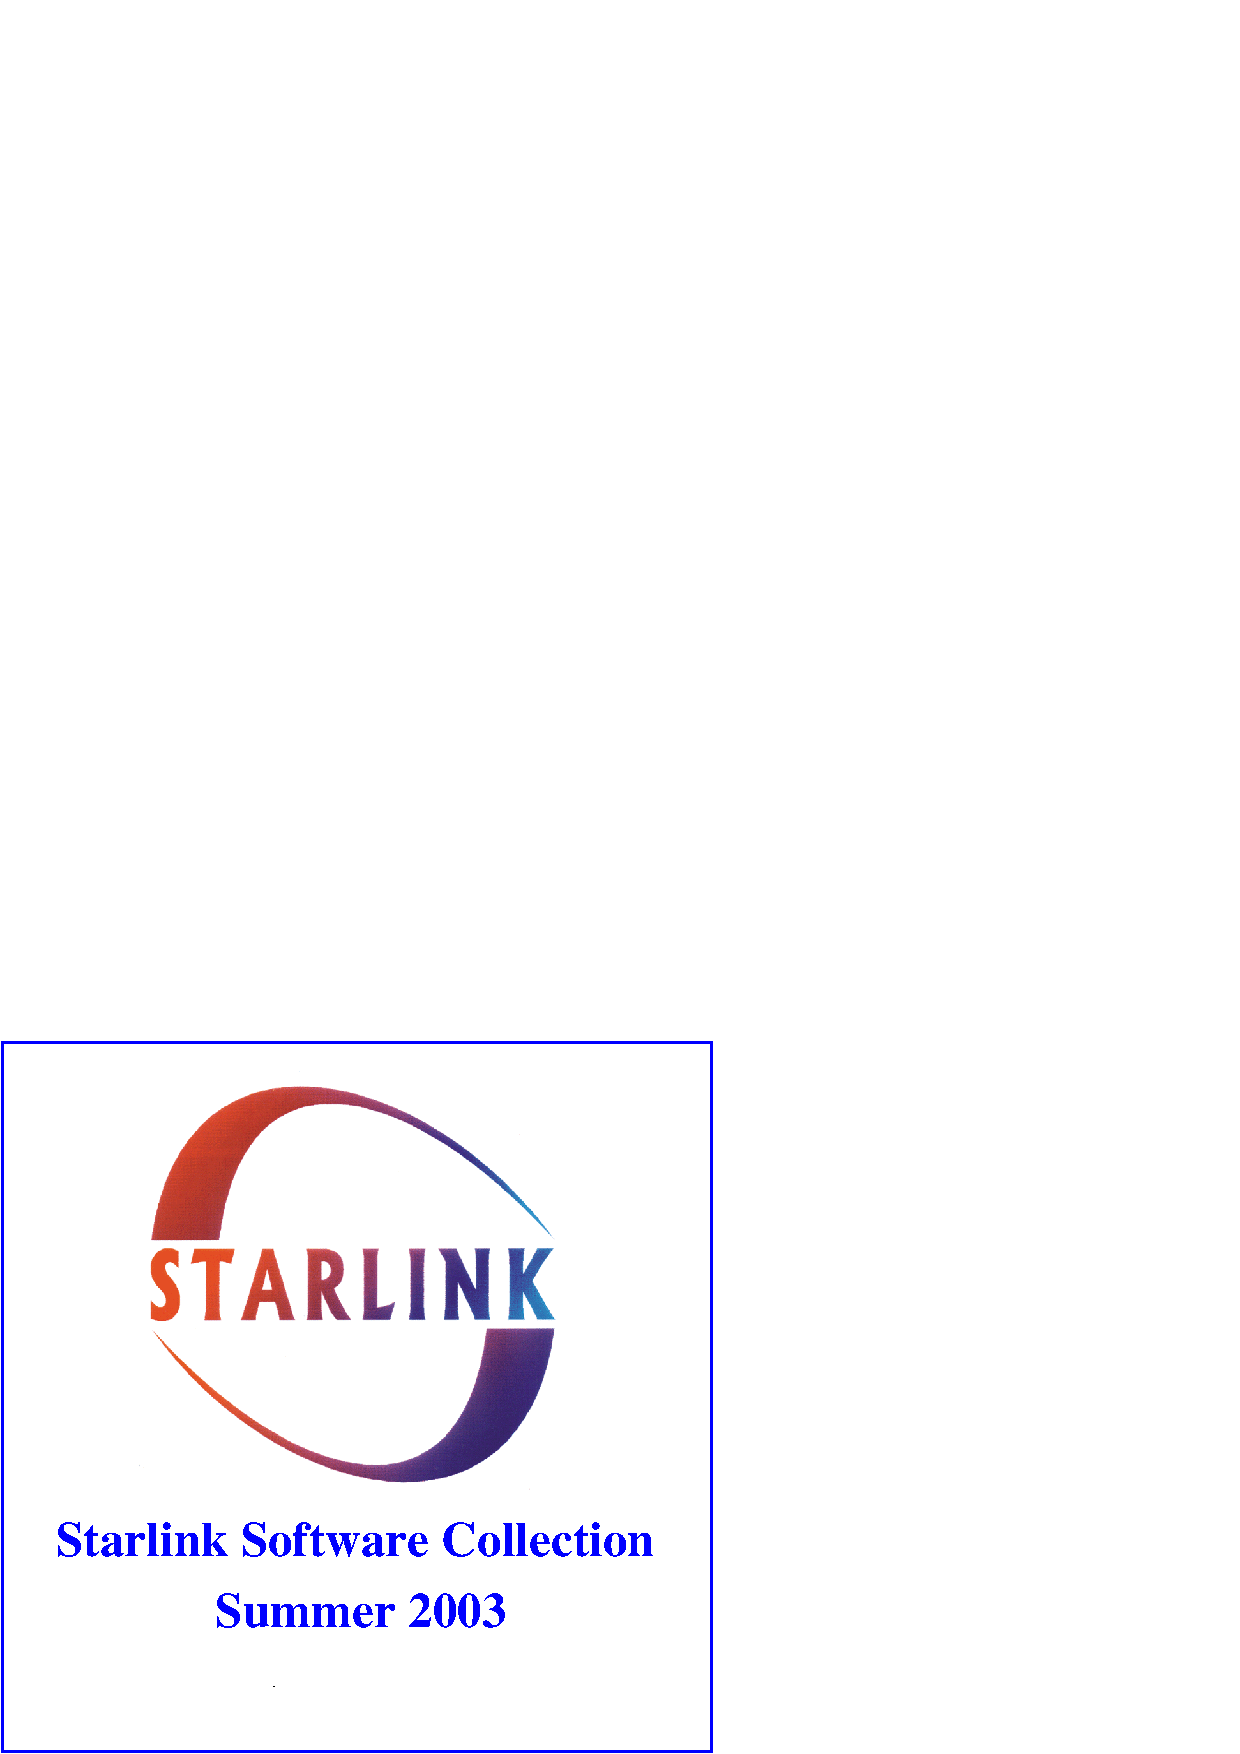
\includegraphics[scale=1.0]{sun212_cover}
% ? End of picture

% ? Heading for abstract if used.
%  \vspace{10mm}
%  \begin{center}
%     {\Large\textbf{Abstract}}
%  \end{center}
% ? End of heading for abstract.

\end{latexonly}

%  HTML documentation header.
%  ==========================
\begin{htmlonly}
   \xlabel{}
   \begin{rawhtml} <H1> \end{rawhtml}
      \stardoctitle\\
      \stardocversion\\
      \stardocmanual
   \begin{rawhtml} </H1> <HR> \end{rawhtml}

% ? Add picture here if required.
  \begin{figure}[h]
  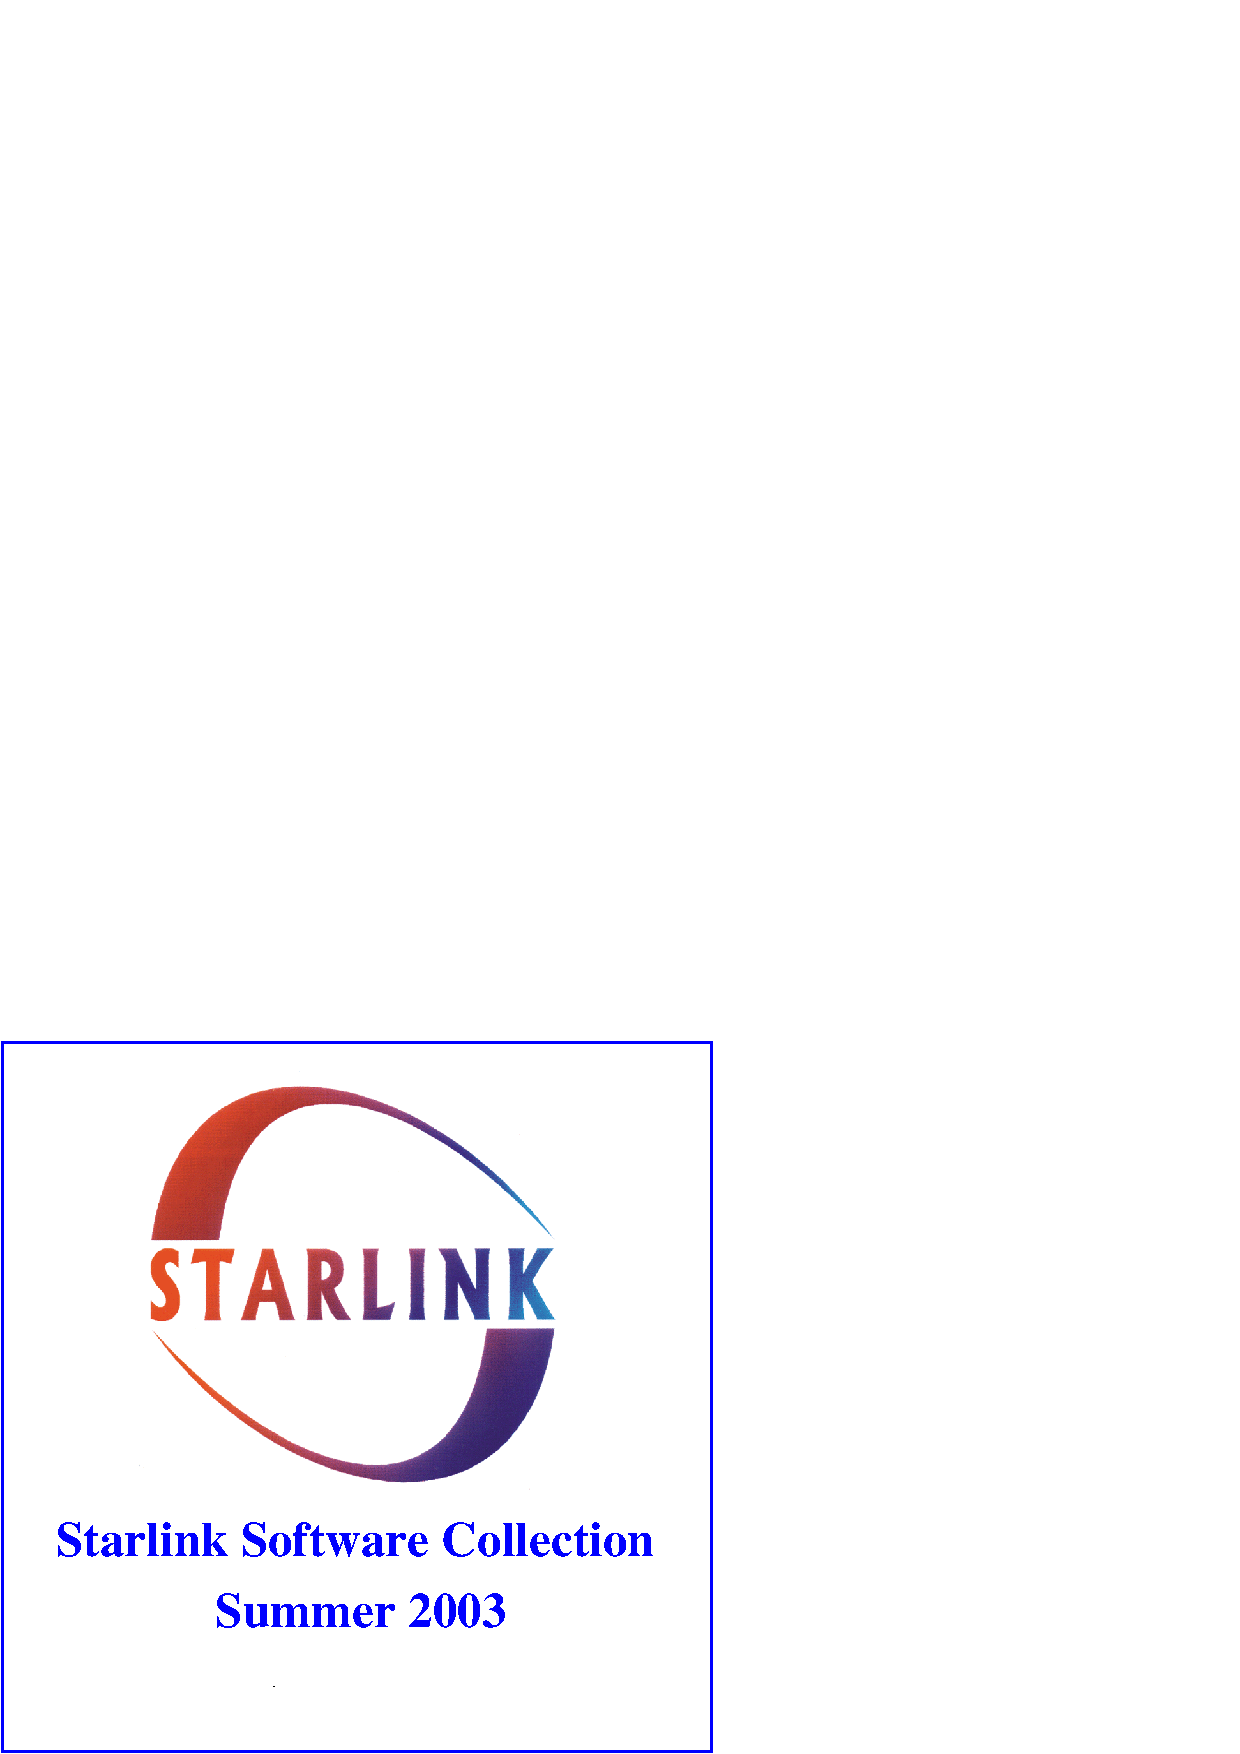
\includegraphics[scale=0.7]{sun212_cover}
  \end{figure}
% ? End of picture

   \begin{rawhtml} <P> <I> \end{rawhtml}
   \stardoccategory\ \stardocnumber \\
   \stardocauthors \\
   \stardocdate
   \begin{rawhtml} </I> </P> <H3> \end{rawhtml}
      \htmladdnormallink{CCLRC / Rutherford Appleton Laboratory}
                        {http://www.cclrc.ac.uk} \\
      \htmladdnormallink{Particle Physics \& Astronomy Research Council}
                        {http://www.pparc.ac.uk} \\
   \begin{rawhtml} </H3> <H2> \end{rawhtml}
      \htmladdnormallink{Starlink Project}{http://www.starlink.ac.uk/}
   \begin{rawhtml} </H2> \end{rawhtml}
   \htmladdnormallink{\htmladdimg{source.gif} Retrieve hardcopy}
      {http://www.starlink.ac.uk/cgi-bin/hcserver?\stardocsource}\\

%  HTML document table of contents.
%  ================================
%  Add table of contents header and a navigation button to return to this
%  point in the document (this should always go before the abstract \section).
  \label{stardoccontents}
  \begin{rawhtml}
    <HR>
    <H2>Contents</H2>
  \end{rawhtml}
  \htmladdtonavigation{\htmlref{\htmladdimg{contents_motif.gif}}
        {stardoccontents}}

% ? New section for abstract if used.
% \section{\xlabel{abstract}Abstract}
% ? End of new section for abstract
\end{htmlonly}

% -----------------------------------------------------------------------------
% ? Document Abstract. (if used)
%  ==================
% \stardocabstract
% ? End of document abstract
% -----------------------------------------------------------------------------
% ? Latex document Table of Contents (if used).
%  ===========================================
  \newpage
  \begin{latexonly}
     \setlength{\parskip}{0mm}
     \tableofcontents
     \setlength{\parskip}{\medskipamount}
     \markboth{\stardocname}{\stardocname}
  \end{latexonly}
% ? End of Latex document table of contents
% -----------------------------------------------------------------------------

% ==============================================================================
% PART 1 - GENERAL
% ==============================================================================

\cleardoublepage
\renewcommand{\thepage}{\arabic{page}}
\setcounter{page}{1}

\begin{latexonly}
\markright{\stardocname}
\end{latexonly}
\part[The Summer 2003 Software \cdroms] %%
{\label{version_of_cdrom}\xlabel{version_of_cdrom} %%
The Summer 2003 Software \cdroms}
\markboth{\stardocname}{\stardocname}

\section{\label{introduction}\xlabel{introduction}Introduction}

This document describes the Summer 2003 distribution of the Starlink
Software for Tru64 Unix, RedHat Linux and Solaris, distributed on
\cdrom.  There are four \cdroms\ available:

\begin{itemize}
\item \axp,
\item \rha,
\item \rhb,
\item \sol.
\end{itemize}

The CDs contain distribution update sets for each package in the
Collection and may be used to update (with the tools provided) existing
installations of the Starlink Software, or to create new tailored
installations.

None of the \cdroms\ contain any actual source code but do contain the
makefiles necessary for package maintenance.  Those readers interested in
obtaining the source code should contact the Starlink Software Librarian
(\htmladdnormallink{\texttt{ussc@star.rl.ac.uk}}{mailto:ussc@star.rl.ac.uk}).

\begin{quote}
\textit{Note: There are no CDs in this release from which the
software will run directly - the Starlink Software has become sufficiently
large that a pared down version to fit on a single CD cannot be produced.}
\end{quote}

%% The Starlink Software will run directly from the runtime \cdroms\ if
%% disk space is short, but performance is critically dependent on the
%% speed of the \cdrom\ drive.  A \cdrom\ drive with a speed of {$24\times$}
%% or better is recommended.

Those readers who received this document after requesting a \cdrom\
distribution will not necessarily have been sent all four CDs, but
should have received the discs relevant to the system(s) on which the
software is intended to run.

%% This may include one or more of the runtime CDs and one of the Update CDs.

\subsection{\xlabel{how_to_use_this_document}How to use this document}
\label{how_to_use_this_document}

This document is divided into two sections as described below.  It is
recommended that you read the descriptions of the parts given below and
then read the remaining parts that are relevant to the installation you
want to create or update.

\subsubsection{Part I -- The Summer 2003 Software \cdroms}

The first part describes the changes to the Starlink software released
with the new issue of the Starlink distribution \cdroms, and gives details
of system requirements for those users new to and/or not familiar with
Starlink software.  It also describes the techniques used to mount \cdroms\
on the various supported systems and the conventions used in this document
and by the tools on the CDs to locate the \cdrom\ once mounted.

\latexhtml{Section~\ref{changes_this_release} (\textit{Changes at this
release}) is particularly relevant to anyone who wants to update an
installation of the Starlink software. }{The
\htmlref{changes}{changes_this_release} section is particularly
relevant to anyone who wants to update an installation of the Starlink
software.}

%% \subsubsection{Part II -- The Runtime \cdroms}

%% The second part describes how to use the runtime \cdroms.

% \textbf{\textit{Note that runtime \cdroms\ are not available for the
% Autumn 1999 distribution.}}

%% You can use the runtime \cdroms\ to create a complete new installation
%% (without source) on local disk, or you can run the Starlink software
%% direct from the \cdrom.   Note that due to space considerations, some
%% of the less popular packages have had to be omitted from the
%% runtime CDs, including CGS4DR.

%% Due to the size of the runtime sets, the documentation is not included on
%% the runtime CDs.  A copy of the runtime documentation set is provided on
%% the \updatesl\ CD for those users able to copy the software to hard disk.

%% If you have an existing installation created from a previous runtime
%% \cdrom\ distribution,  you can update it by completely replacing the
%% old installation with a new runtime distribution or creating a new
%% installation from scratch using the Updates \cdroms.

%% \textbf{You cannot create tailored installations from the runtime \cdroms.}

\subsubsection{Part II -- The \cdroms}

The second part describes how to use the \cdroms.

The \cdroms\ can be used to:

\begin{itemize}
\item update existing Starlink software installations created using previous
issues of the Updates \cdrom,
\item create new installations, tailored to your requirements,
\item install additional software for software development on Linux systems.
\end{itemize}

You cannot run a copy of the Starlink software direct from the \cdroms.

%% If you want to create an installation tailored to your requirements
%% that you can update from future distribution \cdroms, use this method.

\subsection{\xlabel{comments}Comments}
\label{comments}

Please send any comments you may have about this document or the Starlink
Software to the Starlink Software Librarian
(\htmladdnormallink{\texttt{ussc@star.rl.ac.uk}}{mailto:ussc@star.rl.ac.uk}).

\subsection{\xlabel{acknowledgments}\label{acknowledgements}Acknowledgements}

This document has evolved considerably from previous versions.  The author
would like to thank M. J. Bly, Brian McIlwrath (\texttt{bkm@star.rl.ac.uk}), David
Rawlinson and Chris Clayton for their technical contributions and suggestions.


\newpage
\section{\xlabel{Release Notes}Release Notes}
\label{Release_Notes}

\subsection{\xlabel{General Notes}General Notes}

There are two supported operating systems this release (Linux and Solaris).
\textbf{Support for Tru64 Unix has been dropped, but there is still a CD release
containing packages that built and tested OK.} STARJAVA and AUTOASTROM are
not included on the Tru64 CD. No support will be given on problems relating
to applications running under Tru64.

The Linux distribution comes in two flavours this time, Starlink for
RedHat 9.0 and RedHat 7.3. Both CDs will be available.

Like the last release, there is a Starlink CD for Solaris 9.

The DOCS package has been updated and so it must be removed from
your old installation before attempting a software update. ORACDR and
JCMTDR should also be remove before the update is performed. Additionaly
you should remove TREEVIEW, SPLAT JNIHDS and JNIAST first if you select to
install STARJAVA, see below.

Some applications are built with version 2.0 of the astrometry
library AST. While AST 2.0 understands AST's old format for world
co-ordinate systems like the RA \& Dec., earlier AST versions don't
understand the new format. It is recommended that you update all the
packages that are indicated as updates in this release to take advantage
of the new AST. This particularly affects GAIA and KAPPA, where errors
may occur when opening NDFs if the updates are not done.

The \texttt{/star} soft link to your installation directory is now
compulsory. When performing an installation the \texttt{/star}
soft link should be created and the \texttt{INSTALL} and
\texttt{STARLINK} environment variables set to \texttt{/star} before you
start the installation:

\begin{quote}
\begin{verbatim}
% ln -s /path/to/install /star
% setenv INSTALL /star
% setenv STARLINK /star
\end{verbatim}
\end{quote}

\texttt{/path/to/install} is the actual installation directory where
the software will be placed, and should be set to an appropriate
directory that you can write to and that has enough space. You will
need to be root user to create the soft link \texttt{/star}, but after it is
created you should do the installation as the user that can write
to \texttt{/path/to/install} (not root!).

The HTX package has been updated so that the \texttt{findme} and
\texttt{showme} commands work with the Mozilla web browser. To utilise this
feature you must set the \texttt{HTX\_BROWSER} environment variable to
\texttt{mozilla} instead of the default \texttt{netscape}.

\begin{quote}
\begin{verbatim}
% setenv HTX_BROWSER mozilla
\end{verbatim}
\end{quote}

You should now permanently add the \texttt{source /star/etc/login} and
\texttt{source /star/etc/cshrc} commands to your \texttt{\$HOME/.login}
and \texttt{\$HOME/.cshrc} files respectively:

\begin{quote}
\begin{verbatim}
In $HOME/.cshrc

if (-e /star/etc/cshrc ) then
   source /star/etc/cshrc
endif

In $HOME/.login

if (-e /star/etc/login ) then
   source /star/etc/login
endif
\end{verbatim}
\end{quote}

\subsection{\xlabel{star-java}STARJAVA}

The Starlink Java Software (STARJAVA) has had numerous changes and
additions. STARJAVA can now be considered as a separate entity from
the classic Starlink applications and libraries, although in this
release it is provided as a standard Starlink package. TREEVIEW, SPLAT
JNIHDS and JNIAST have been moved to STARJAVA, if you need the updates to
these packages then you must first deinstall the old versions before
installing STARJAVA.

STARJAVA can be run from the CD-ROM if you have the Java Runtime
Environment (JRE) v1.4 (or greater) and Java Advanced Imaging (JAI)
1.1\_2-rc (or greater) installed. The software will still run without
the JAI but with reduced functionality. All the files in the distribution
of STARJAVA are in the directory \texttt{starjava} on the CD-ROM.
Running the software from the CD-ROM will work for the Solaris, Linux
and Windows operating systems. There are five applications
that you can run, SOG, SPLAT, FROG, TREEVIEW and TABLECOPY. To run
the applications you need to supply the \texttt{jar} filename for
the application to the \texttt{java} command:

\begin{quote}
\begin{verbatim}
For Unix

% java -jar /path/to/cdrom/starjava/lib/sog/sog.jar           (SOG)
% java -jar /path/to/cdrom/starjava/lib/splat/splat.jar       (SPLAT)
% java -jar /path/to/cdrom/starjava/lib/frog/frog.jar         (FROG)
% java -jar /path/to/cdrom/starjava/lib/treeview/treeview.jar (TREEVIEW)
% java -jar /path/to/cdrom/starjava/lib/table/table.jar       (TABLECOPY)
\end{verbatim}
\end{quote}

\texttt{/path/to/cdrom/} is the path to the top level of you mounted CD-ROM.

\begin{quote}
\begin{verbatim}
For Windows

c:\> java -jar D:\starjava\lib\sog\sog.jar           (SOG)
c:\> java -jar D:\starjava\lib\splat\splat.jar       (SPLAT)
c:\> java -jar D:\starjava\lib\frog\frog.jar         (FROG)
c:\> java -jar D:\starjava\lib\treeview\treeview.jar (TREEVIEW)
c:\> java -jar D:\starjava\lib\table\table.jar       (TABLECOPY)
\end{verbatim}
\end{quote}
\texttt{D:} is the letter of your CD-ROM drive.

The \texttt{java} command must be on your path for any of these commands to work.
See the document \xref{}{sun251}{} \texttt{Getting Started with the Starlink
Java Infrastructure and Applications Set} for further details on command
line switches that can be used with the applications.

If you experience problems with JRE v1.4.1\_02 distributed with
RedHat 9.0 CD, such as problems with the Java Plugin for Mozilla,
or Java crashes (SIGSEGV). Then a possible cure is to set the
environment variable \texttt{LD\_ASSUME\_KERNEL}:

\begin{quote}
\begin{verbatim}
% setenv LD_ASSUME_KERNEL 2.4.1
\end{verbatim}
\end{quote}

\subsection{\xlabel{quickin}quick\_install Script}

There is a new installation tool on the CD-ROM this time called \texttt{quick\_install}.
This tool can be run directly from the CD-ROM to do a full fresh installation of
the Starlink Software. It can not be used for updating existing installations.
The script requires root access to create the soft link \texttt{/star}.

When running the script you will be asked to supply the full path to the
desired installation directory and to the CD-ROM. The CD-ROM must be mounted!
It will also ask you if you would like to setup the Starlink news service,
but this can be skipped if you are installing a personal copy of the software,
as it is only used for site wide installations.

Basically, just follow the prompts given by the script and you will have a
full installation as quickly as possible.

The \texttt{quick\_install} script creates an install log in your home directory,

\begin{quote}
\begin{verbatim}
% $HOME/quick_log
\end{verbatim}
\end{quote}

This will be useful to diagnose problems if the installation should fail.

\subsection{\label{windows}\xlabel{windows}STARJAVA for Microsoft Windows}

There is a Microsoft Windows version of STARJAVA which can be downloaded from \\
\htmladdnormallink{\texttt{ftp://ftp.starlink.ac.uk/pub/ussc/windows/starjava.exe}}{ftp://ftp.starlink.ac.uk/pub/ussc/windows/starjava.exe}
and is also included on the Starlink CD-ROM in directory \texttt{windows}.
To install STARJAVA just run the executable and you will be presented with a standard
Windows graphical installer. You will have the options to install all applications and
documentation, plus the Java Runtime Environment (JRE) and Java Advanced Imaging (JAI).
JRE and JAI have their own installers, but these are started by the STARJAVA installer
(if they are selected for installation). A full installation of everything is approximately
191 Mb. You will also be presented with the option to select the installation directory.
Desktop icons (optional) and Start Menu Icons will be created with links to the
GUI applications and documentation. See the document \xref{}{sun251}{}
\texttt{Getting Started with the Starlink Java Infrastructure and Applications Set}
for further details.

\section{\xlabel{conditions_of_use}Conditions of Use}
\label{conditions_of_use}

Starlink has recently revised the conditions of use of the Starlink
software. The software is still distributed free of distribution charge,
but is now under GPL License.

\begin{quote}
\latexonlysmall
\begin{center}\textbf{STARLINK SOFTWARE COPYRIGHT}\end{center}

\textbf{PREAMBLE}

The purpose of this document is to state the terms and conditions
under which Starlink software, documentation, data and other associated
material (``the Software'') may be used.

\par
\textbf{NOTICE TO USER:}
\par
\textbf{BY USING THE SOFTWARE YOU ACCEPT THE FOLLOWING TERMS AND CONDITIONS
WHICH APPLY TO ITS USE.}

\begin{enumerate}

\item The Starlink Software Collection is Copyright 1980-2003, Council
 for the Central Laboratory of the Research Councils (``CCLRC''),
 except where noted internally, or discussed below.

\item The Starlink Project has recently made the decision to license its
 own software under the GNU General Public License (GPL) as published
 by the Free Software Foundation; either version 2 of the License,
 or (at your option) any later version. However, this transition is
 not, and may never be, complete, and the following points should be
 borne in mind.

  * All the code produced by the Starlink Project itself
    is copyright CCLRC and is distributed under the terms of the GPL.

  * Some software packages include a CONDITIONS statement which
    refers to, or contains the text within, $<$\ldots$>$.
    These are also
    copyright CCLRC and this conditions statement should be taken
    to refer instead to the GPL.

  * Some packages include third-party code which is either non-GPL
    code or whose copyright and licence status is unclear.  These
    packages are therefore not (or not clearly) GPL.

  * Some packages consist largely of code donated in gentler times,
    when issues of copyright and licences were unimportant and
    largely unrecorded.  For these packages, some or all of the
    licence, copyright and even authorship is unknown, but they
    cannot be safely taken to be public domain.  You can safely
    assume only that they have a broad `academic use only' licence.
    This set of packages includes at least Figaro.

\item If you wish to use the code for a purpose for which the licence
 conditions, authorship or copyright are important, you should
 consult the project at \texttt{ussc@star.rl.ac.uk}.

\item This Software is distributed in the hope that it will be useful, but
 WITHOUT ANY WARRANTY; without even the implied warranty of
 MERCHANTABILITY or FITNESS FOR A PARTICULAR PURPOSE. See the GNU General
 Public License for more details.

\item You should have received a copy of the GNU General Public License along
 with this Software; if not, write to the Free Software Foundation, Inc.,
 51 Franklin Street, Fifth Floor, Boston, MA 02110-1301 USA. You can also find
 the GPL on the GNU web site.

\item Some of the code distributed here refers to an earlier version of
 the Starlink Software Licence, located at
 \htmladdnormallink{\texttt{http://www.starlink.ac.uk/store/conditions.html}}{http://www.starlink.ac.uk/store/conditions.html},
 which permitted non-commercial use only.  This licence has been
 superseded, and any references to that licence should be taken to
 refer to this licence instead.

\item In addition, we ask you to consider acknowledging the Collection in any
 program or publication in which you use it.  For general publications,
 we suggest `The authors acknowledge the data analysis facilities
 provided by the Starlink Project which is run by CCLRC on behalf
 of PPARC.'
\end{enumerate}
\end{quote}

\begin{quote}
\latexonlysmall
\begin{center}\textbf{GNU General Public License}\end{center}

\begin{center}
{\parindent 0in

Version 2, June 1991

Copyright \copyright\ 1989, 1991 Free Software Foundation, Inc.

\bigskip

59 Temple Place - Suite 330, Boston, MA  02111-1307, USA

\bigskip

Everyone is permitted to copy and distribute verbatim copies
of this license document, but changing it is not allowed.
}
\end{center}

\begin{center}
{\bf\large Preamble}
\end{center}


The licenses for most software are designed to take away your freedom to
share and change it.  By contrast, the GNU General Public License is
intended to guarantee your freedom to share and change free software---to
make sure the software is free for all its users.  This General Public
License applies to most of the Free Software Foundation's software and to
any other program whose authors commit to using it.  (Some other Free
Software Foundation software is covered by the GNU Library General Public
License instead.)  You can apply it to your programs, too.

When we speak of free software, we are referring to freedom, not price.
Our General Public Licenses are designed to make sure that you have the
freedom to distribute copies of free software (and charge for this service
if you wish), that you receive source code or can get it if you want it,
that you can change the software or use pieces of it in new free programs;
and that you know you can do these things.

To protect your rights, we need to make restrictions that forbid anyone to
deny you these rights or to ask you to surrender the rights.  These
restrictions translate to certain responsibilities for you if you
distribute copies of the software, or if you modify it.

For example, if you distribute copies of such a program, whether gratis or
for a fee, you must give the recipients all the rights that you have.  You
must make sure that they, too, receive or can get the source code.  And
you must show them these terms so they know their rights.

We protect your rights with two steps: (1) copyright the software, and (2)
offer you this license which gives you legal permission to copy,
distribute and/or modify the software.

Also, for each author's protection and ours, we want to make certain that
everyone understands that there is no warranty for this free software.  If
the software is modified by someone else and passed on, we want its
recipients to know that what they have is not the original, so that any
problems introduced by others will not reflect on the original authors'
reputations.

Finally, any free program is threatened constantly by software patents.
We wish to avoid the danger that redistributors of a free program will
individually obtain patent licenses, in effect making the program
proprietary.  To prevent this, we have made it clear that any patent must
be licensed for everyone's free use or not licensed at all.

The precise terms and conditions for copying, distribution and
modification follow.

\begin{center}
{\Large \sc Terms and Conditions For Copying, Distribution and
  Modification}
\end{center}

\begin{enumerate}

\addtocounter{enumi}{-1}

\item

This License applies to any program or other work which contains a notice
placed by the copyright holder saying it may be distributed under the
terms of this General Public License.  The ``Program'', below, refers to
any such program or work, and a ``work based on the Program'' means either
the Program or any derivative work under copyright law: that is to say, a
work containing the Program or a portion of it, either verbatim or with
modifications and/or translated into another language.  (Hereinafter,
translation is included without limitation in the term ``modification''.)
Each licensee is addressed as ``you''.

Activities other than copying, distribution and modification are not
covered by this License; they are outside its scope.  The act of
running the Program is not restricted, and the output from the Program
is covered only if its contents constitute a work based on the
Program (independent of having been made by running the Program).
Whether that is true depends on what the Program does.

\item You may copy and distribute verbatim copies of the Program's source
  code as you receive it, in any medium, provided that you conspicuously
  and appropriately publish on each copy an appropriate copyright notice
  and disclaimer of warranty; keep intact all the notices that refer to
  this License and to the absence of any warranty; and give any other
  recipients of the Program a copy of this License along with the Program.

You may charge a fee for the physical act of transferring a copy, and you
may at your option offer warranty protection in exchange for a fee.

\item

You may modify your copy or copies of the Program or any portion
of it, thus forming a work based on the Program, and copy and
distribute such modifications or work under the terms of Section 1
above, provided that you also meet all of these conditions:

\begin{enumerate}

\item

You must cause the modified files to carry prominent notices stating that
you changed the files and the date of any change.

\item

You must cause any work that you distribute or publish, that in
whole or in part contains or is derived from the Program or any
part thereof, to be licensed as a whole at no charge to all third
parties under the terms of this License.

\item
If the modified program normally reads commands interactively
when run, you must cause it, when started running for such
interactive use in the most ordinary way, to print or display an
announcement including an appropriate copyright notice and a
notice that there is no warranty (or else, saying that you provide
a warranty) and that users may redistribute the program under
these conditions, and telling the user how to view a copy of this
License.  (Exception: if the Program itself is interactive but
does not normally print such an announcement, your work based on
the Program is not required to print an announcement.)

\end{enumerate}


These requirements apply to the modified work as a whole.  If
identifiable sections of that work are not derived from the Program,
and can be reasonably considered independent and separate works in
themselves, then this License, and its terms, do not apply to those
sections when you distribute them as separate works.  But when you
distribute the same sections as part of a whole which is a work based
on the Program, the distribution of the whole must be on the terms of
this License, whose permissions for other licensees extend to the
entire whole, and thus to each and every part regardless of who wrote it.

Thus, it is not the intent of this section to claim rights or contest
your rights to work written entirely by you; rather, the intent is to
exercise the right to control the distribution of derivative or
collective works based on the Program.

In addition, mere aggregation of another work not based on the Program
with the Program (or with a work based on the Program) on a volume of
a storage or distribution medium does not bring the other work under
the scope of this License.

\item
You may copy and distribute the Program (or a work based on it,
under Section 2) in object code or executable form under the terms of
Sections 1 and 2 above provided that you also do one of the following:

\begin{enumerate}

\item

Accompany it with the complete corresponding machine-readable
source code, which must be distributed under the terms of Sections
1 and 2 above on a medium customarily used for software interchange; or,

\item

Accompany it with a written offer, valid for at least three
years, to give any third party, for a charge no more than your
cost of physically performing source distribution, a complete
machine-readable copy of the corresponding source code, to be
distributed under the terms of Sections 1 and 2 above on a medium
customarily used for software interchange; or,

\item

Accompany it with the information you received as to the offer
to distribute corresponding source code.  (This alternative is
allowed only for noncommercial distribution and only if you
received the program in object code or executable form with such
an offer, in accord with Subsection b above.)

\end{enumerate}


The source code for a work means the preferred form of the work for
making modifications to it.  For an executable work, complete source
code means all the source code for all modules it contains, plus any
associated interface definition files, plus the scripts used to
control compilation and installation of the executable.  However, as a
special exception, the source code distributed need not include
anything that is normally distributed (in either source or binary
form) with the major components (compiler, kernel, and so on) of the
operating system on which the executable runs, unless that component
itself accompanies the executable.

If distribution of executable or object code is made by offering
access to copy from a designated place, then offering equivalent
access to copy the source code from the same place counts as
distribution of the source code, even though third parties are not
compelled to copy the source along with the object code.

\item
You may not copy, modify, sublicense, or distribute the Program
except as expressly provided under this License.  Any attempt
otherwise to copy, modify, sublicense or distribute the Program is
void, and will automatically terminate your rights under this License.
However, parties who have received copies, or rights, from you under
this License will not have their licenses terminated so long as such
parties remain in full compliance.

\item
You are not required to accept this License, since you have not
signed it.  However, nothing else grants you permission to modify or
distribute the Program or its derivative works.  These actions are
prohibited by law if you do not accept this License.  Therefore, by
modifying or distributing the Program (or any work based on the
Program), you indicate your acceptance of this License to do so, and
all its terms and conditions for copying, distributing or modifying
the Program or works based on it.

\item
Each time you redistribute the Program (or any work based on the
Program), the recipient automatically receives a license from the
original licensor to copy, distribute or modify the Program subject to
these terms and conditions.  You may not impose any further
restrictions on the recipients' exercise of the rights granted herein.
You are not responsible for enforcing compliance by third parties to
this License.

\item
If, as a consequence of a court judgment or allegation of patent
infringement or for any other reason (not limited to patent issues),
conditions are imposed on you (whether by court order, agreement or
otherwise) that contradict the conditions of this License, they do not
excuse you from the conditions of this License.  If you cannot
distribute so as to satisfy simultaneously your obligations under this
License and any other pertinent obligations, then as a consequence you
may not distribute the Program at all.  For example, if a patent
license would not permit royalty-free redistribution of the Program by
all those who receive copies directly or indirectly through you, then
the only way you could satisfy both it and this License would be to
refrain entirely from distribution of the Program.

If any portion of this section is held invalid or unenforceable under
any particular circumstance, the balance of the section is intended to
apply and the section as a whole is intended to apply in other
circumstances.

It is not the purpose of this section to induce you to infringe any
patents or other property right claims or to contest validity of any
such claims; this section has the sole purpose of protecting the
integrity of the free software distribution system, which is
implemented by public license practices.  Many people have made
generous contributions to the wide range of software distributed
through that system in reliance on consistent application of that
system; it is up to the author/donor to decide if he or she is willing
to distribute software through any other system and a licensee cannot
impose that choice.

This section is intended to make thoroughly clear what is believed to
be a consequence of the rest of this License.

\item
If the distribution and/or use of the Program is restricted in
certain countries either by patents or by copyrighted interfaces, the
original copyright holder who places the Program under this License
may add an explicit geographical distribution limitation excluding
those countries, so that distribution is permitted only in or among
countries not thus excluded.  In such case, this License incorporates
the limitation as if written in the body of this License.

\item
The Free Software Foundation may publish revised and/or new versions
of the General Public License from time to time.  Such new versions will
be similar in spirit to the present version, but may differ in detail to
address new problems or concerns.

Each version is given a distinguishing version number.  If the Program
specifies a version number of this License which applies to it and ``any
later version'', you have the option of following the terms and conditions
either of that version or of any later version published by the Free
Software Foundation.  If the Program does not specify a version number of
this License, you may choose any version ever published by the Free Software
Foundation.

\item
If you wish to incorporate parts of the Program into other free
programs whose distribution conditions are different, write to the author
to ask for permission.  For software which is copyrighted by the Free
Software Foundation, write to the Free Software Foundation; we sometimes
make exceptions for this.  Our decision will be guided by the two goals
of preserving the free status of all derivatives of our free software and
of promoting the sharing and reuse of software generally.

\begin{center}
{\Large\sc
No Warranty
}
\end{center}

\item
{\sc Because the program is licensed free of charge, there is no warranty
for the program, to the extent permitted by applicable law.  Except when
otherwise stated in writing the copyright holders and/or other parties
provide the program ``as is'' without warranty of any kind, either expressed
or implied, including, but not limited to, the implied warranties of
merchantability and fitness for a particular purpose.  The entire risk as
to the quality and performance of the program is with you.  Should the
program prove defective, you assume the cost of all necessary servicing,
repair or correction.}

\item
{\sc In no event unless required by applicable law or agreed to in writing
will any copyright holder, or any other party who may modify and/or
redistribute the program as permitted above, be liable to you for damages,
including any general, special, incidental or consequential damages arising
out of the use or inability to use the program (including but not limited
to loss of data or data being rendered inaccurate or losses sustained by
you or third parties or a failure of the program to operate with any other
programs), even if such holder or other party has been advised of the
possibility of such damages.}

\end{enumerate}


\begin{center}
{\Large\sc End of Terms and Conditions}
\end{center}


\pagebreak[2]

\subsection{Appendix: How to Apply These Terms to Your New Programs}

If you develop a new program, and you want it to be of the greatest
possible use to the public, the best way to achieve this is to make it
free software which everyone can redistribute and change under these
terms.

  To do so, attach the following notices to the program.  It is safest to
  attach them to the start of each source file to most effectively convey
  the exclusion of warranty; and each file should have at least the
  ``copyright'' line and a pointer to where the full notice is found.

\begin{quote}
one line to give the program's name and a brief idea of what it does.
Copyright (C) yyyy  name of author

This program is free software; you can redistribute it and/or modify
it under the terms of the GNU General Public License as published by
the Free Software Foundation; either version 2 of the License, or
(at your option) any later version.

This program is distributed in the hope that it will be useful,
but WITHOUT ANY WARRANTY; without even the implied warranty of
MERCHANTABILITY or FITNESS FOR A PARTICULAR PURPOSE.  See the
GNU General Public License for more details.

You should have received a copy of the GNU General Public License
along with this program; if not, write to the Free Software
Foundation, Inc., 59 Temple Place - Suite 330, Boston, MA  02111-1307, USA.
\end{quote}

Also add information on how to contact you by electronic and paper mail.

If the program is interactive, make it output a short notice like this
when it starts in an interactive mode:

\begin{quote}
Gnomovision version 69, Copyright (C) yyyy  name of author \\
Gnomovision comes with ABSOLUTELY NO WARRANTY; for details type `show w'. \\
This is free software, and you are welcome to redistribute it
under certain conditions; type `show c' for details.
\end{quote}


The hypothetical commands {\tt show w} and {\tt show c} should show the
appropriate parts of the General Public License.  Of course, the commands
you use may be called something other than {\tt show w} and {\tt show c};
they could even be mouse-clicks or menu items---whatever suits your
program.

You should also get your employer (if you work as a programmer) or your
school, if any, to sign a ``copyright disclaimer'' for the program, if
necessary.  Here is a sample; alter the names:

\begin{quote}
Yoyodyne, Inc., hereby disclaims all copyright interest in the program
`Gnomovision' (which makes passes at compilers) written by James Hacker.

signature of Ty Coon, 1 April 1989 \\
Ty Coon, President of Vice
\end{quote}


This General Public License does not permit incorporating your program
into proprietary programs.  If your program is a subroutine library, you
may consider it more useful to permit linking proprietary applications
with the library.  If this is what you want to do, use the GNU Library
General Public License instead of this License.
\end{quote}
%\begin{quote}
%\latexonlysmall
%\begin{center}\textbf{STARLINK SOFTWARE LICENCE}\end{center}
%
%\textbf{PREAMBLE}
%
%The purpose of this document is to state the terms and conditions
%under which Starlink software, documentation, data and other associated
%material (``the Software'') may be used.
%\par
%\textbf{NOTICE TO USER:}
%\par
%\textbf{BY USING THE SOFTWARE YOU ACCEPT THE FOLLOWING TERMS AND CONDITIONS
%WHICH APPLY TO ITS USE.}
%
%\begin{enumerate}
%\item  The Software is owned by the Council for the Central Laboratory of the
%Research Councils (``CCLRC'') unless a statement to the contrary appears
%within the Software itself.
%
%\item The Software is made available free of charge for use in teaching and
%research by:
%\begin{enumerate}
%\item private individuals for non-profit research; and
%\item non-profit educational, academic and research institutions.
%\end{enumerate}
%
%\item Commercial use of the Software is specifically excluded from the terms
%and conditions of this licence.  Commercial use of the Software is subject
%to the prior written agreement of CCLRC on terms to be agreed.
%
%\item The provision of any version of the Software under the terms and
%conditions specified herein does not imply that future versions will also
%be made available under the same terms and conditions.
%
%\item The user may modify the Software for his own purposes.  The user may
%distribute the modified software provided that CCLRC is informed and that
%a copy of the modified software is made available to CCLRC on request.
%All modifications made by the user shall be clearly identified to show how
%the modified software differs from the original Software.
%
%\item In any published work produced by the user and which includes results
%achieved by using the Software, the user shall acknowledge that the Software
%was used in producing the information contained in such publication.
%
%\item The user may incorporate or embed the Software into other software
%products which he may then give away free of charge but not sell provided
%the user makes due acknowledgement of the use which he has made of the
%Software in creating such software products.   Any redistribution of the
%Software in this way shall be made under the same terms and conditions
%under which the user received it from CCLRC.
%
%\item The user shall not cause the Software to be brought into disrepute,
%either by misuse, or use for inappropriate tasks, or by inappropriate
%modification.
%
%\item The Software is provided to the user ``as is'' and CCLRC makes no
%warranty as to its suitability or performance.   CCLRC does not and
%cannot warrant the performance or results which the user may obtain by
%using the Software.  CCLRC makes no warranties, express or implied, as
%to non-infringement of third party rights, merchantability, or fitness
%for any particular purpose.  In no event will CCLRC be liable to the
%user for any consequential, incidental, or special damages, including
%any lost profits or lost savings, even if a CCLRC representative has
%been advised of such damages, or for any claim by any third party.
%
%\end{enumerate}
%\end{quote}

\newpage
\section{\xlabel{changes_this_release}Changes at this release}
\label{changes_this_release}

This section details changes to the Starlink packages at this release.
All packages in the distribution have been rebuilt from a common source set.
Details of each \cdrom\ are described in later sections.  A list of all
the packages is available in appendix~\ref{available_software}, and tables
of the sizes of installed packages are available in
appendix~\ref{package_sizes}.

\subsection{\xlabel{new_packages}New packages}
\label{new_packages}

The following new packages are available in this release.

\begin{description}

%\item[HDSTOOLS] is a suite of utilities for editing, inspecting and manipulating
%HDS files.  The new document -- \textit{\xref{HDSTOOLS -- Tools To Display and Edit
%HDS Objects}{sun245}{}\/} (SUN/245) describes the package.

\item[AUTOASTROM v0.5-7] Autoastrometry of mosaics. The new document (SUN/242)
\textit{\xref{AUTOASTROM -- Autoastrometry for Mosaics}{sun242}{}\/}
describes the package. AUTOASTROM is not available under Tru64 Unix.

\item[JCMTDR v1.2-2] Applications for reducing JCMT GSD on-the-fly data.
The documents SC/1 \textit{\xref{JCMTDR Cookbook}{sc1}{}\/} and
SUN/132 \textit{\xref{Applications for Reducing JCMT GSD Data 1.2-2 User's manual}{sun132}{}\/}
describe the package.

\item[STARJAVA v1.0b] Starlink Java Infrastructure and Applications Set.
The new document (SUN/251)
\textit{\xref{Getting Started with the Starlink Java Infrastructure
and Applications Set}{sun251}{}\/}
describes the package and \texttt{/star/starjava/javadocs/index.html}
describes the Starlink STARJAVA classes API. There are miscellaneous
documents in \texttt{/star/starjava/docs/} for individula package information and
third party application documentation.

The STARJAVA package contains the following applications and classes. Note,
SPLAT, TREEVIEW, JNIAST and JNIHDS have been moved to the STARJAVA
package, instead of being individual packages.

\begin{description}
\item[APPLICATIONS/UTILITIES in STARJAVA]
\item[ FROG V0.1a] Display and analysis of time series data (new)
\item[ SOG V0.1] Son of GAIA (new)
\item[ SPLAT V2.0] Spectral Analysis Tool (update)
\item[ TABLECOPY V0.3] Copy tables from one format to another (new)
\item[ TOPCAT V0.3b] Tool for OPerations on Catalogues and Tables (new)
\item[ TREEVIEW V2.1-3] Hierarchical data viewer (update)

\item[CLASS LIBRARIES in STARJAVA]
\item[ ARRAY V0.2] N-dimensional array manipulation and I/O (new)
\item[ ASTGUI V1.0] AST specific UI components (new)
\item[ AXIS V1.0b2] Third generation Apache SOAP (new)
\item[ COCO V1.0] Java UI for Coco (new)
\item[ DOM4J V0.1] Third party DOM access library (org.dom4j.*) (new)
\item[ FITS V0.1] STARJAVA-specific FITS access (new)
\item[ HDS V0.1] Non-native HDS utility classes (new)
\item[ HDX V0.1] A flexible, extensible, data model for astronomical images,
tables and other metadata (new)
\item[ JAIUTIL V1.0] Utility classes for JAI (new)
\item[ JETTY V4.0.4] HTTP Server and Servlet Container (new)
\item[ JNIAST V2.0-4] Java Native interface to AST (update)
\item[ JNIHDS V0.3] Java Native Interface to HDS (update)
\item[ JSKY V2.0] Java Components for Astronomy (new)
\item[ JUNIT V3.7] Third party unit testing framework (junit.*) (new)
\item[ NDX V0.1] N-dimensional astronomical object manipulation and I/O (new)
\item[ PAL V0.1] Positional Astronomy Library (new)
\item[ RV V1.0] Java UI for RV (new)
\item[ TABLE V0.3] Generic table manipulation and I/O (new)
\item[ TAMFITS V0.93] Third party basic FITS access (nom.tam.*) (new)
\item[ UTIL V0.1] Miscellaneous utillity classes (new)
\item[ VOTABLE V1.0] VOTable I/O (new)
\end{description}

The STARJAVA package can be considered to be independent of the standard USSC,
and in future will be distributed separately. All the STARJAVA applications
and classes are distributed under the GPL licence.

The SPLAT documentation (SUN/243) \textit{\xref{SPLAT - A Spectral Analysis
Tool}{sun243}{}\/} has been updated and can be found in
\texttt{/star/starjava/docs/splat/sun243.htx/sun243.html}. It also appears
in the DOCS package and can be seen with the command \texttt{showme sun243}.

STARJAVA is not available under Tru64 Unix.

\end{description}


\subsection{\xlabel{application_and_utility_updates}Application and utility updates}
\label{application_and_utility_updates}

\begin{description}
\item[ASTROM v3.7] Update - Now reports its astrometry information additionally
through generated FITS WCS headers (this is still provisional, see the notes on this
topic in the documentation, SUN/5). There are new arguments on the command line,
allowing you to request a summary and log files (the latter easily parseable).

\item[ATOOLS v1.5] Update - New commands added: \texttt{astinvert}, \\
\texttt{astmapbox}, \texttt{astspecframe}, \texttt{astsetrefpos} and \texttt{astgetrefpos}.
These are straight analogues of the corresponding AST routines. When reading or writing AST objects,
ATOOLS commands now indicate the nature of the file accessed (i.e. whether it is an NDF,
a FITS file or a text file).

\item[CCDPACK v4.0-15] Fix - Release v4.0-15 is a bug fix update of CCDPACK

\item[CONVERT v1.5] Update - \texttt{SPECX2NDF} has been revamped so that it now uses
the new AST SpecFrame functionality. \texttt{FITS2NDF} converts INES archive IUE
spectra. Improved propagation of existing world co-ordinate system (WCS)
headers in \texttt{NDF2FITS}.

\item[DIPSO v3.6-1] Update - The \texttt{READ} command has been modified so that it will
attempt to read spectral axis information from the WCS component of an NDF.
The \texttt{WRITE} command has been modified so that it will add a WCS component to the
output NDF describing the spectral axis.

\item[EXTRACTOR v1.4-2] Fix - is a bug fix release.

\item[FIGARO v5.6-2] Fix - is a bug fix release.

\item[GAIA v2.6-12] Update - A number of new catalogues and image servers are now available.
New configuration options \texttt{``-extended\_precision''} and \texttt{``-show\_hdu\_chooser''} have
been added. The pixel table now highlights the maximum and minimum values. The
command-line options of GAIA can be configured using the new
\texttt{``File''-$>$ ``Startup options''} window. Plus several bug fixes.

\item[KAPPA v1.1-1]  Update - Added initial support for spectral world coordinate systems
(see \texttt{WCSADD}, \texttt{LINPLOT}, etc). This includes flexible conversion between different
units, spectral systems and reference frames.

\item[ORAC-DR v4.0-1] Update - Support for UIST and INGRID in all observation modes.
Support for ISAAC in imaging mode, and preliminary support for spectroscopy mode.
Four new recipes including \texttt{NOD\_SKY\_FLAT\_THERMAL} recipe for reduction of thermal data
using sky observations for flat-fielding. Plus many other updates and fixes.

\item[PERIOD v5.0-2] Fix - is a bug fix release.

\item[PISA v2.4-5] Fix - is a bug fix release.

\item[POLPACK v3.1-2] Update - Minor Updates.

\item[SPECX v6.8-1] Update - New Commands: \texttt{SET-DATA-DIRECTORY} and \texttt{SWITCH-DATE}.
Plus several bug fixes.

\item[SURF v1.6-11] Fix - is a bug fix release.

\end{description}

\subsection{\xlabel{new_infrastructure}New infrastructure}
\label{new_infrastructure}

None.

%There is one new infrastructure package in this distribution:

%\begin{description}

%\item[JNIHDS] is a Java Native Interface for the HDS library.
%(`showme jnihds\_doc' on Starlink systems).

%\end{description}

\subsection{\xlabel{infrastructure_updates}Infrastructure updates}
\label{infrastructure_updates}

There has been a number of infrastructure updates since the previous
release.

\begin{description}
\item[AST v2.0-9] Update - The implementation of the \texttt{astWrite} \texttt{(AST\_WRITE)}
function within the \texttt{FitsChan} class has been modified. Support for spectral
coordinate systems has been introduced through the addition of two new classes,
\texttt{SpecFrame} and \texttt{SpecMap}. Facilities have been added to the \texttt{Frame}
class which allow differences in axis units to be taken into account when finding a Mapping
between two Frames. Various bug fixes.
\item[CFITSIO v2.4.40b] Update - The CFITSIO function library v2.4.40b is now
available.

\item[EMS v2.0-7] Fix - Various bug fixes.

\item[HTX v1.2-7] Update - Added Mozilla web browser capability. Bug fixes.

\item[GRP v3.2] Update - Shell meta-characters may now be included with file
specifications.

\item[IFD v1.2-8] Fix - Various bug fixes.

\item[IMG v1.3-1] Update - FITS character strings may now be free-format. Bug
fix.

\item[INIT v1.1-24] Update - Command definitions for AUTOASTROM, JCMTDR
and STARJAVA added.

\item[JRE v1.4.1\_02] Update - Java Runtime Environment v1.4.1\_02 and Java
Advanced Imaging v1\_1\_2-rc.

\item[KAPLIBS v2.3] Update - \texttt{kpg1\_dsfrm} modified to include details of \\
AST SpecFrames. \texttt{kpg1\_asmrg} modified to attempt alignment in Domain SPECTRAL.
Script \texttt{kaplibs\_link added} for linking standalone applications. \texttt{GETHLP}
moved from KAPPA to \texttt{KAPLIBS:KAPGEN}.

\item[MERS v1.8] Update - \texttt{MSG1\_GREF} is completely revised to simplify its interface
with the parameter system, using a new routine \texttt{SUBPAR\_GREF}. Plus bug fixes.

\item[MESSGEN v1.1-3] Fix - Bug fixes.

\item[PCS v4.1-1] Update - A new subroutine \texttt{SUBPAR\_GREF} provides the functionality
required by the MERS routine \texttt{MSG1\_GREF}. Plus bug fixes.

\item[PERL v5.8.0] Update - The Starlink installation of PERL is at Perl V5.8.0.

\item[PERLMODS v1.5-0] Update - Numerous module updates and the new modules
Astro-FITS-CFITSIO-1.01, Inline-0.44, Parse-RecDescent-1.94, Pod-Escapes-1.03,
Pod-Simple-0.96, Text-Balanced-1.94 and Tk-HistEntry-0.40.

\item[PGPLOT v5.2.2-2] Update - Bug fixes and updates from the original PGPLOT source.

\item[PRIMDAT v1.3-1] Fix - Bug fixes.

\item[PSX v0.4] Update - Added \texttt{PSX\_PUTENV}, \texttt{PSX\_\_NOMEM} to \texttt{psx\_err} and
\texttt{TEST\_PUTENV} routines.

\item[SLALIB v2.4-11] Update - A new routine \texttt{PLANTU} has been added.
Documentation updates.

\item[STAR2HTML v1.4-6] Fix - Bug fixes.

\item[STARPERL v1.4] Update - Updates to Starlink::Config v1.00, NDF v1.45,
Starlink v1.14, GSD v1.13 and Astro-SLA v0.96.
\end{description}

\subsection{\xlabel{base_set_updates}Base set updates}
\label{base_set_updates}

There are no changes to the base set at this release.

\subsection{\xlabel{withdrawn_packages}Withdrawn Packages}
\label{withdrawn_packages}

There are no packages withdrawn at this release.

\subsection{New, updated or withdrawn documents}

This section lists documents not directly related to particular packages that
have been updated or withdrawn.  This section also contains details of documents
related to software not available on the \cdroms\ that have been updated
or withdrawn.

\paragraph{New documents:}

%There are no new documents at this release.

\begin{itemize}
\item \textit{\xref{SUN/246.01 ORAC-DR - integral field spectroscopy data
reduction 4.0 User Guide (NEW)}{sun246}{}\/}

\item \textit{\xref{SUN/251.01 STARJAVA - Getting Started with the Starlink Java
Infrastructure and Applications Set (NEW)}{sun251}{}\/}

\item \textit{JAVADOCS/1.0b STARJAVA - \texttt{/star/starjava/javadocs/index.html} -\\
Starlink STARJAVA classes API (NEW)}

\end{itemize}


\paragraph{Updated documents:}

\begin{itemize}
\item \textit{\xref{SUN/001.23 STARLINK Software Collection}{sun1}{}\/}
\item \textit{\xref{SUN/005.18 ASTROM - Basic astrometry program}{sun5}{}\/}
\item \textit{\xref{SUN/050.24 DIPSO - A friendly spectrum analysis program}{sun50}{}\/}
\item \textit{\xref{SUN/055.19 CONVERT - A Format-conversion Package}{sun55}{}\/}
\item \textit{\xref{SUN/067.61 SLALIB - Positional Astronomy Library}{sun67}{}\/}
\item \textit{\xref{SUN/095.23 KAPPA - Kernel Application Package}{sun95}{}\/}
\item \textit{\xref{SUN/109.11 PISA - Position Intensity and Shape Analysis}{sun109}{}\/}
\item \textit{\xref{SUN/121.05 PSX - POSIX interface routines}{sun121}{}\/}
\item \textit{\xref{SUN/132.03 JCMTDR - Applications for Reducing JCMT GSD Data}{sun132}{}\/}
\item \textit{\xref{SUN/150.06 GRP - Routines for Managing Groups of Objects}{sun150}{}\/}
\item \textit{\xref{SUN/160.06 IMG - Simple Image Data Access}{sun160}{}\/}
\item \textit{\xref{SUN/193.06 PERL - Practical Extraction and Report Language}{sun193}{}\/}
\item \textit{\xref{SUN/210.12 AST - World Coordinate System library (Fortran)}{sun210}{}\/}
\item \textit{\xref{SUN/211.12 AST - World Coordinate Systems library (C version)}{sun211}{}\/}
\item \textit{\xref{SUN/212.12 Starlink Software CD-ROMs Summer 2003 User's Guide}{sun212}{}\/}
\item \textit{\xref{SUN/214.13 GAIA - Graphical astronomy \& image analysis tool}{sun214}{}\/}
\item \textit{\xref{SUN/216.08 SURF - SCUBA User Reduction Facility}{sun216}{}\/}
\item \textit{\xref{SUN/227.02 Disk FITS input/output functions}{sun227}{}\/}
\item \textit{\xref{SUN/228.05 STARPERL - Starlink Perl modules}{sun228}{}\/}
\item \textit{\xref{SUN/230.05 ORAC-DR - Overview and General Introduction}{sun230}{}\/}
\item \textit{\xref{SUN/232.07 ORAC-DR - imaging data reduction v1.0 user's guide}{sun232}{}\/}
\item \textit{\xref{SUN/236.03 ORAC-DR - spectroscopy data reduction}{sun236}{}\/}
\item \textit{\xref{SUN/238.03 KAPLIBS - Internal subroutines used within KAPPA}{sun238}{}\/}
\item \textit{\xref{SUN/243.02 SPLAT - Moved to DOCS package}{sun243}{}\/}
\end{itemize}

\paragraph{Withdrawn documents:}

SUN/244 - TREEVIEW deleted.

\subsection{News items}

The \cdroms\ contain a directory of news items which gives some
details of the new versions and bug fixes available (see
section~\ref{installation_cdrom_contents}).

\subsection{\xlabel{data_protection}Data protection}
\label{data_protection}

Due to the requirements of the UK Data Protection Act 1998, we are
required to exercise caution in distributing personal data to any country
which does not have Data Protection laws or which has Data Protection
laws which are less stringent than those in the UK.

We have therefore decided to cease CD distribution of the data files
of Starlink user's names and email addresses, and the world lists of
astronomers and observatories, as of the Spring 2000 distribution.
Both sets of files will continue to be available to UK starlink sites
via a private distribution mechanism.

Other users may query the world list of astronomers by using the
\htmladdnormallink{Astrosearch}{http://www.starlink.ac.uk/astrolist/astrosearch.html}
utility on the Starlink Web server\latex{~at
\texttt{http://www.starlink.ac.uk/astrolist/astrosearch.html}}.

\subsection{Size changes}

The size of a complete installation is approximately 2.0Gb.

\newpage
\section{\xlabel{system_requirements}System requirements}
\label{system_requirements}

The following sections give details of the requirements necessary for
Compaq Alpha/Tru64 Unix, PC/RedHat Linux and SUN SPARC/Solaris
systems to run the Starlink Software.

% \textit{The disk space requirements listed below for \textbf{runtime} systems
% listed below apply to the Spring 1999 \cdrom.  There are no runtime
% \cdroms for the Autumn 1999 distribution.}

\subsection{\xlabel{dec_alpha_digital_unix}Compaq Alpha / Tru64 Unix}
\label{dec_alpha_digital_unix}

The requirements for an Alpha/Tru64 Unix system to run the Starlink Software
are as follows:

\begin{itemize}

\item System -- Any Compaq Alpha system with a minimum of 128Mb memory
running Tru64 Unix v5.1 or higher.  It should have swap space 2-3
times larger than its physical memory.  Total virtual memory should be
adequate for your data processing needs.

\textbf{It is known that this build will not run on versions of Tru64
Unix earlier than v5.0.}

\item Disk -- A complete installation requires \axpfull.
A basic system with one or two packages plus run-time support requires
from 2Mb to 50Mb.  A more extensive system with several large packages
requires from 100Mb to 200Mb.   Additional space is required for user
data.  A 3Gb disk or partition is the recommended minimum if you wish
to install the whole collection.

\item Compilers -- The Starlink Software for Tru64 Unix was built
with the v5.5 Tru64 Unix Fortran Compiler set using the v402 run-time
library set.  It is known that this build will not run under some older
versions of the Compiler libraries and run-time library.  The C++ runtime
libraries (v6.5) are required for GAIA and CURSA.

\end{itemize}

\subsection{\xlabel{intel_pc_linux}PC / RedHat Linux}
\label{intel_pc_linux}

The requirements for a PC/RedHat Linux computer to use the Starlink Software
are as follows:

\begin{itemize}

\item Processor -- Intel compatible PC with Pentium or higher
processor.  A Pentium II class processor or above is highly recommended.

\item Memory -- 64Mb minimum, 128Mb recommended.  Swap space should be
2-3 times larger than the physical memory. Total virtual memory should be
adequate for your data processing needs.

\item Disk -- A complete installation requires \rhafull.
A basic system with one or two packages plus run-time support requires
from 2Mb to 50Mb.  A more extensive system with several large packages
requires from 100Mb to 200Mb.   Additional space is required for user
data.  A 3Gb disk or partition is the recommended minimum if you wish
to install the whole collection.

\item Linux -- There are two Linux versions of the Starlink Software,
one built under RedHat Linux 7.3 using the 2.4.18 kernel and the other
built under RedHat Linux 9.0 using the 2.4.20 kernel.

RedHat Linux 7.3 is the Linux distribution supported by Starlink but it
should also be possible to run the Software on any Linux distribution
that has \texttt{glibc} v2.2 support (see later).

It is not recomended that the Linux RedHat 9.0 version be used
on Linux distributions with  \texttt{glibc} $<$ v2.3.2.

\textbf{The Summer 2003 \cdroms\ will not run on RedHat Linux
distributions earlier than v7.1.} Please see the section
\htmlref{\textit{Problems on Linux Systems}}{problems_on_linux_systems}
\latex{(Section~\ref{problems_on_linux_systems})} for details of problems
that may be encountered on Linux systems.

\item Compilers -- The Starlink software for Linux uses the
\texttt{gcc} C and Fortran integrated compiler sets.  In addition the
\texttt{g++} compiler is used for parts of GAIA and CURSA.  Appropriate
versions of these compilers and associated libraries are provided on
the \cdroms.

\item C RTL (Run Time Library) -- The packages on the Summer 2003
updates \cdrom\ were built with the GNU C Library shared library at
version 2.2.5 (RedHat 7.3) and version 2.3.2 (RedHat 9.0).

\end{itemize}

\subsection{\xlabel{sun_sparc_solaris}SUN SPARC / Solaris}
\label{sun_sparc_solaris}

The requirements for a SUN SPARC / Solaris system to run the Starlink Software
are as follows:

\begin{itemize}

\item System -- Any SUN SPARC system with a minimum of 128Mb memory running
Solaris 8.  The build was done under Solaris 9.  If the machine is used
by others or for processing large amounts of data, it should have swap
space 2-3 times larger than its physical memory.

\textbf{The software will NOT run on Solaris v7 and earlier
due to changes to support 64bit file addressing and other system library
changes.}

\item Disk -- A complete installation off \cdrom\ requires \solfull.
A basic system with one or two packages plus run-time support requires
from 2Mb to 50Mb.  A more extensive system with several large packages
requires from 100Mb to 200Mb.   Additional space is required for user
data.  A 3Gb disk or partition is the recommended minimum if you wish
to install the whole collection.

\item Compilers -- The Starlink Software for Solaris was built with the
Workshop v6 Update 2 Compilers.  Where possible, binaries have been statically
linked to allow the software to run on systems without the Fortran compiler
libraries installed but in some cases the v6.2 SPARC Compiler shared
libraries will be required.

\item Libraries -- Apart from the standard system libraries and the
compiler libraries mentioned above, some systems (CCDPACK and XRV
GUIs, GAIA) may be dynamically linked with the OpenWindows X libraries.
You will need either the standard OpenWindows shared libraries or one of
the MIT X11 shared library sets to run these.

\end{itemize}

\subsection{\xlabel{general_requirements}General requirements}
\label{general_requirements}

The Starlink software initialisation system is designed to run from the
C-shell via \texttt{login} and \texttt{cshrc} resources scripts.  This means
that you need either the standard C-shell or tc-shell to run the
Starlink software.  ORAC-DR requires tc-shell.

\newpage
\section{\xlabel{mounting_the_cdroms}Mounting the \cdroms}
\label{mounting_the_cdroms}

The \cdroms\ are written in \texttt{iso9660} format and so should be
mounted as described in the following sections.  It is assumed that you
are logged in as \texttt{root} and are using the Bourne shell
\texttt{sh} (Tru64 Unix or Solaris) or Bourne--Again SHell
\texttt{bash} (Linux).

\subsection{\xlabel{mounting_on_alpha}Mounting on Tru64 Unix systems}
\label{mounting_on_alpha}

This section describes mounting on Tru64 Unix systems.

On Tru64 Unix systems, you must have support for \texttt{iso9660} format CDs
in the system kernel.  You require the line:

\begin{quote}
\begin{verbatim}
options       CDFS
\end{verbatim}
\end{quote}

in your \texttt{/sys/conf/SYSTEM\_NAME} kernel configuration file.  You should
rebuild and reinstall your kernel if required.

The instructions below assume the device name of the \cdrom\ drive is
\texttt{/dev/rz4c}.  This may differ on your machine.

To mount the \cdrom\ at boot time add the following entry to your
\texttt{/etc/fstab} file:

\begin{quote}
\begin{verbatim}
/dev/rz4c   /cdrom cdfs   ro,rrip  0 0
\end{verbatim}
\end{quote}

This assumes you have a mount point directory \texttt{/cdrom}.

You can then mount the \cdrom\ by issuing the following commands:

\begin{quote}
\begin{verbatim}
# mkdir /cdrom
# mount -at cdfs
\end{verbatim}
\end{quote}

To mount the \cdrom\ without an entry in \texttt{/etc/fstab}, you can issue
the commands:

\begin{quote}
\begin{verbatim}
# mkdir /cdrom
# mount -t cdfs -o ro,rrip /dev/rz4c /cdrom
\end{verbatim}
\end{quote}

which will create a mount point \texttt{/cdrom} and mount the disk on it.

\subsection{\xlabel{mounting_on_linux}Mounting on Linux systems}
\label{mounting_on_linux}

RedHat Linux creates mount points under the \texttt{/mnt} directory for
the floppy disk drive and the \cdrom\ drive if they exist.  The entry for
\cdrom\ in the \texttt{/etc/fstab} file should have an entry
similar to this:

\begin{quote}
\begin{verbatim}
/dev/scd0      /mnt/cdrom                iso9660 -r,exec 0 0
\end{verbatim}
\end{quote}

The device name \texttt{/dev/scd0} may vary depending on your system.  The
\texttt{exec} option is necessary to allow you to run binaries and
scripts from the \cdrom.   The tools on the CDs will not run if you do not
use this option.

If a \cdrom\ is already mounted, then you should first dismount it
(being careful to ensure that you are not currently in a subdirectory
of the mounted \cdrom):

\begin{quote}
\begin{verbatim}
# umount /mnt/cdrom
\end{verbatim}
\end{quote}

The Starlink \cdrom\ can then be inserted and mounted by issuing the command:

\begin{quote}
\begin{verbatim}
# mount /mnt/cdrom
mount: block device /dev/scd0 is write-protected, mounting read-only
\end{verbatim}
\end{quote}
The message you get just tells you that the \cdrom\ is read only.

If for some reason the above does not work, you can mount the \cdrom\ by
hand on a mount-point by issuing the command:

\begin{quote}
\begin{verbatim}
# mkdir /cdrom
# mount -r -t iso9660 -o exec /dev/scd0 /cdrom
\end{verbatim}
\end{quote}

where \texttt{/dev/scd0} is the device name of a SCSI \cdrom\ drive and
\texttt{/cdrom} is the mount-point.

\subsection{\xlabel{mounting_on_solaris}Mounting on Solaris systems}
\label{mounting_on_solaris}

If your system has the Volume Manager running, the \cdrom\ should be
automatically mounted under \texttt{/cdrom/cdrom0} when it is inserted
into the drive.  If you are not running the Volume Manager, then you
will need to mount the disc manually with the following command:

\begin{quote}
\begin{verbatim}
# mkdir /mnt
# mount -F hsfs -r /dev/dsk/c0t6d0s2 /mnt
\end{verbatim}
\end{quote}

This will mount the \cdrom\ under \texttt{/mnt}.  Note that the device
name \texttt{/dev/dsk/c0t6d0s2} is the default under Solaris but
may be different on your system, depending on your hardware
configuration.

If a \cdrom\ is already mounted, then you should first dismount it
(being careful to ensure that you are not currently in a subdirectory
of the mounted \cdrom).  If the Volume Manager is runhaning, you can do
this with the command:

\begin{quote}
\begin{verbatim}
# eject cdrom0
\end{verbatim}
\end{quote}

This will automatically unmount the \cdrom\ and eject it from the drive.
Note that on some non--standard hardware set--ups, the command may be
\texttt{eject cd} or \texttt{eject cd0}.

If the Volume Manager is not running, then the command to unmount the
\cdrom\ (assuming that it is mounted under \texttt{/mnt}) is:

\begin{quote}
\begin{verbatim}
# umount /mnt
\end{verbatim}
\end{quote}

You will need to manually eject the \cdrom\ (usually with the eject
button on the front of the \cdrom\ drive).

\subsection{\xlabel{mount__via_nfs}Mounting via NFS from another system}
\label{mount_via_nfs}

\textit{This method of providing access to the \cdroms\ has been known
to cause problems with the update tool, preventing it from unpacking some
of the distribution sets on the \cdroms.  Remote mounhating is
not recommended unless unavoidable.}

If you do not have a local \cdrom\ drive you can install the
software by mounting the CD via NFS\@.  The \cdrom\ should be mounted as
appropriate on a remote Unix system and then made available for NFS
export.

In these examples, the file system exported from the remote system,
\texttt{machine}, is the directory \texttt{/cdrom}.  Mount the exported
CD on a mount--point you have created \textsl{e.g.} \texttt{/cdrom}.

For Tru64 Unix and Linux, the \texttt{mount}  command is:

\begin{quote}
\begin{verbatim}
# mount -r -t nfs machine:/cdrom /cdrom
\end{verbatim}
\end{quote}

On Solaris systems, remote mounting other file systems via NFS is more
complicated and best left to a System Manager to arrange.  Ideally,
the remote exported \cdrom\ should be available on your machine via the
automount system.

\subsection{\xlabel{cdrom_conventions}\cdrom\ conventions}
\label{cdrom_conventions}

The previous sections contain the details of how to mount the \cdroms\ on
various systems.  Each system has a different method and mount points may
vary considerably.

Therefore in the remainder of this document the environment variable
\texttt{CDROM} is used to specify the mount point of the \cdrom.  This
is defined thus:

\begin{quote}
\begin{verbatim}
# CDROM='/mnt/cdrom' ; export CDROM
\end{verbatim}
\end{quote}

in Bourne or Bash shell, and

\begin{quote}
\begin{verbatim}
% setenv CDROM /mnt/cdrom
\end{verbatim}
\end{quote}

in C-shell or tc-shell.

\textbf{This environment variable is important because the remainder of this
document assumes that it exists and the tools on the
\cdroms\ will not run without it.}


% ==============================================================================
% PART 2 - CD-ROMS
% ==============================================================================
\newpage
%\cleardoublepage
\begin{latexonly}
\markright{\stardocname}
\end{latexonly}
%%  \addtocontents{toc}{\protect\clearpage}  % Page throw for table of contents
\part[The installation \cdroms]{\xlabel{installation_cdrom}The Installation \cdroms}
\label{installation_cdrom}
\markboth{\stardocname}{\stardocname}

\section{\xlabel{installation_cdrom_introduction}Introduction}
\label{installation_cdrom_introduction}

The installation \cdroms\ are only distribution
media -- you cannot run the Starlink software directly off them.
They contain the software sets required to create new installations of
the Starlink software and the tools required to update existing
installations.

The \axp\ and \sol\ \cdroms\ contains the base set installation kits.

The \rha\ and \rhb\ \cdroms\ contains the set of compilers and associated
packages for Linux.

The following sections describe the contents of the \cdroms, what
options are available for using them, and the tools provided.

The methods for installing or updating are then described in separate
sections and apply to all version of the \cdroms.

\subsection{\xlabel{installation_cdrom_contents}Installation \cdrom\ contents}
\label{installation_cdrom_contents}

The \cdroms\ have the following files and directories:

\begin{quote}
\rha\ and \rhb
\begin{verbatim}
% ls $CDROM
CONDITIONS.html  README_FIRST.html  README_JAVA
docs  INSTALL  linux_bits  news  packages  quick-install
Summer-2003  starjava  tools  windows
\end{verbatim}
\axp\ and \sol:
\begin{verbatim}
% ls $CDROM
CONDITIONS.html  README_FIRST.html  README_JAVA
Summer-2003  docs  packages  quick-install  INSTALL
base  news  starjava  tools  windows
\end{verbatim}
\end{quote}

The contents are as follows:
starjava  Summer-2003  tools  windows
\begin{itemize}

\item \texttt{README\_FIRST.html} -- Index to the documentation on the CD-ROM.

\item \texttt{README\_JAVA} -- A brief installation guide for STARJAVA under
                               Microsoft Windows and instructions on how to
                               run STARJAVA from the CD-ROM (Windows and Unix).

\item \texttt{starjava} -- A directory containing runtime STARJAVA files, see
                           the README\_JAVA file.

\item \texttt{windows} -- A directory containing the Windows STARJAVA installation
                          files (starjava.exe)

\item \texttt{CONDITIONS.html} -- The distribution and use conditions which
you must read.

\item \texttt{INSTALL} -- A brief installation guide and release notes.

\item \texttt{Summer-2003} -- An empty file to tag the distribution.

\item \texttt{base} (\axp\ and \sol)-- Contains the Base Set software
for Tru64 Unix and Solaris.  The Base Set is a collection of widely
available utilities recommended for use at Starlink sites in the UK and
provided on the \cdrom\ as a means of distribution.

\item \texttt{docs} -- Contains a copy of the hypertext for this document.

\item \texttt{linux-bits} (\rha\ and \rhb) -- Extra bits and pieces
for Linux required for program development, such as the versions of the
compilers used to build the Starlink software under Linux.

\item \texttt{news} -- News items for Starlink sites which use the
Starlink NEWS utility.  The file \texttt{\$CDROM/news/news\_ussc.txt}
gives a summary of the Summer 2003 software release.

\item \texttt{packages} -- `runtime' software sets for all the
available applications, libraries and utilities.  These sets do not
contain the source code but do contain the makefiles used for building
the packages.

\item \texttt{tools} -- Various tools for installations and updates.


\item \texttt{quick\_install} -- A tool for doing a full installation of the
Starlink Software (should not be used for updating existing systems).

\end{itemize}

The following sections contain recipes for updating existing software
installations and creating new ones.

\subsection{\xlabel{using_the_cdroms}Using the \cdroms}
\label{using_the_cdroms}

The \cdroms\ give you the ability to update your existing
installation of Starlink Software or to install a new tailored
installation.  Which you choose to use depends upon your requirements.

\begin{itemize}

\item If your existing installation is well maintained and reasonably
up-to-date, you should probably choose to update it.  This includes
installations created from previous Updates \cdroms.

\item If your existing installation has lots of software packages
installed for which this distribution does not provide updates, you
should update the installation rather than start from scratch.
This category includes most UK Starlink sites.

\item If your installation is old and has not been updated since you got
it, or has got out-of-date, or has not been well maintained, you should
scrap it and start from scratch either with a fresh installation tailored
to your requirements, or a full installation.

\item If you do not have an existing installation you have no choice but to
create a new one.

\end{itemize}

\begin{quote}
\textbf{NOTE:}~Existing installations which pre-date the Autumn 1997
Starlink \cdrom\ distributions cannot be updated from this distribution
due to changes made in the installation directory structure for the
Autumn 1997 distribution.

If you have an installation that pre-dates the Autumn 1997
distributions, you should consider scraping it and installing a new
installation, or obtaining the Autumn 1997 and subsequent Updates
\cdroms\ and using those distributions to bring your old installation
into a state where this distribution may be used to update it.  This
option entails a lot of work and great care and is not recommended.

Starting from scratch is the preferred option.
\end{quote}

\subsubsection{Updating an existing installation}

Updating your installation gives you the opportunity to update as many
packages as you want within your existing installation.

If you have packages installed for which no update is available, you
should update the rest of your installation to get the updated packages
rather than start from scratch.  You can check the inventory of software
for which updates are provided in the appendix on
\htmlref{available software}{available_software} \latex{(see appendix
\ref{available_software})}.

Most UK Starlink Sites and sites that have recently installed complete
Starlink software installations from \cdrom\ should consider updating
their existing installations.

\subsubsection{\xlabel{starting_from_scratch}Starting from scratch}
\label{starting_from_scratch}

Starting from scratch allows you to tailor a software installation to your
requirements with complete control over what you have installed, or to
make a complete installation of the whole system without worrying about what
is available.

If your Starlink software installation was obtained before the Autumn
1997 \cdrom\ distribution you should consider starting again, unless
you have software installed for which there are no update sets in this
distribution.

If you \emph{do} have packages installed for which there are no
update sets in this distribution, you can elect to start from scratch,
but you will have to take steps to deinstall those packages before you
create your new installation and then reinstall them once your new
installation is on line.

\subsection{\xlabel{tools_on_the_cdrom}Tools on the \cdrom}
\label{tools_on_the_cdrom}

There are two tools on the \cdroms\ to make it easy to install packages
and to do some of the more complex administration tasks required for
this release.

The \texttt{remove} tool is used to tidy up the installation before doing
the main update.  It can also be used to remove packages from an installation.

The \texttt{update} tool has been developed to make updating software
packages in an existing installation easy.  The tool allows you to
update the whole of your existing installation in one run, to update
sets of software (libraries, utilities, examples) or to update packages
one by one.  The tool is also used to install packages on new systems.

The \texttt{update} tool does NOT preserve old versions of the software packages it
updates -- you are advised to make copies of any key software packages
in your existing installation before you begin the update.  There is no
tool for reinstating old versions of software packages though it is possible
to reinstall old copies from previous Updates CDs.

There are a number of dependencies within the Starlink software.  This
means that if you update or install a package, you may at the same
time have to update or install the other packages that it depends on.
The tool is NOT aware of these dependencies which are listed in the
\htmlref{dependencies section}{software_dependencies}
\latex{(see appendix~\ref{software_dependencies})}.
The order of installing dependent packages does not generally matter except
that HTX must be installed first for new installations.

\newpage

\section{\xlabel{updating_an_existing_installation}Updating an existing installation}
\label{updating_an_existing_installation}

This section tells you how to update existing Starlink software
installations created with the Autumn 2002 Updates \cdrom\ distribution.
The intended audience is the UK Starlink Sites and those sites with
tailored installations who wish to update rather than replace their
existing installation.

Sites that have installations based on the Spring 2000 runtime \cdrom\
distributions should replace it with a new
\htmlref{tailored installation}{installing_from_scratch} (see
section~\ref{installing_from_scratch}).

The general sequence of events is as follows:

\begin{enumerate}

\item \textbf{Pre-update tasks}.  This first step in the process
is to check the installation and to make various necessary changes that
then allow the update to proceed smoothly.

\item \textbf{Update the installation}.  The second step is the update
itself which can be done all at once or staggered to meet your site
requirements.

You can update as much or as little as you want at each `pass', from
a single package to whole groups of packages depending on how adventurous
you are.  If you need to keep selected applications running at their
old versions `just in case' while a researcher completes a data
reduction program, this can be done but you should remember that if you
update some packages, you must install the updates for those it depends
upon.  In general Starlink packages are backwards compatible but since this
is a major new release some tasks are not.

\end{enumerate}

The instructions in the sections that follow assume that you are the
owner of the Starlink software installation you intend to update.

\subsection{\xlabel{pre-update_tasks_and_setups}Pre-update tasks and setups}
\label{pre-update_tasks_and_setups}

The pre-update tasks can be broken down into sets:

\begin{enumerate}
\item mount the appropriate \cdrom, set environment variables, and warn users,
\item remove obsolete documentation and packages if any,
\item check for beta-test installations,
\item remove the old \texttt{package\_updated} flag files,
\item update packages requiring a special sequence.
\end{enumerate}

The following sections describe the pre-update tasks in more detail.  You
must complete each task before proceeding to update your installation.

It is assumed that you execute these tasks as the owner of the
existing Starlink software installation, except where noted.
Use of C-shell or tc-shell is assumed.

\subsubsection{Mounting the \cdrom\ and setting environment variables}

The first step is to \htmlref{mount}{mounting_the_cdrom} the appropriate
\cdrom\ \latex{(see section~\ref{mounting_the_cdroms})}
and set some environment variables as follows:

\begin{enumerate}

\item Mount the appropriate \cdrom\ and check that you have the
environment variable \texttt{CDROM} set as described in
section~\ref{cdrom_conventions}.  You may need to be \texttt{root} to
mount the \cdrom.

You should mount the \axp\ or \rha\ or \rhb\ or \sol\ \cdrom\ to update a Tru64
Unix, Linux, or Solaris installation.

\item Set \texttt{SYSTEM} to indicate which system you are updating:
\texttt{alpha\_OSF1} for Tru64 Unix, \texttt{ix86\_Linux} for Linux
or \texttt{sun4\_Solaris} for Solaris (\emph{e.g.,} \texttt{`setenv SYSTEM
ix86\_Linux'}).

\item Set \texttt{INSTALL} to indicate the root directory of your
installation.  This is most often \texttt{/star} but may be any absolute
directory name (\emph{e.g.,} \texttt{`setenv INSTALL /star'}). It
is now compulsory to have /star as a real directory or as a soft
link to your installation directory. For this reason we recommend
that you do a fresh install.

\item If your \texttt{INSTALL} variable is set to something other than
\texttt{/star}, you must set the variable \texttt{STARLINK} to be the
same as \texttt{INSTALL} (\emph{e.g.,} \texttt{`setenv STARLINK \$INSTALL'}).

\item At Starlink sites where the Starlink NEWS package is used to
proved a news service for users, you need to set various environment
variables to define the local print command, the local contact name and
contact email address:

\begin{itemize}
\item Set \texttt{LOCALPRINT} to define the print command used by the
`Print' option in NEWS.
\item Set \texttt{MAINTAINER} to the administrator of the NEWS system.
\item Set \texttt{NEWSEMAIL} to the administrator's email address.
\end{itemize}

If you do not wish to install the Starlink PERL set you should set the
\texttt{PERL} environment variable to point to an appropriate Perl
installation.   \textbf{Note:} the ORAC-DR pipeline system requires the
Starlink PERL installation and the PERLMODS and STARPERL packages so if
you wish to install ORAC-DR, please install PERL, PERLMODS and STARPERL too.

The two sets of quotes are important in these definitions.

\begin{quote}
\begin{verbatim}
% setenv LOCALPRINT '"lpr -P0"'
% setenv MAINTAINER '"Your name"'
% setenv NEWSEMAIL '"Your email address"'
% setenv PERL /wherever/perl
\end{verbatim}
\end{quote}

\item Those people updating installations used by multiple users should warn
the users that the updates are about to take place because while the updates
take place, the whole installation will be disrupted.

How you warn your users is up to you.  The update process can take
anything from a few minutes for small installations with just a few
packages to an hour or more for full installations.  Update time also
depends on how fast your processor/disk system is.

\end{enumerate}

\subsubsection{Removing obsolete documents and hypertext}

There are a number of old documents not distributed with particular
packages that have been withdrawn from the Starlink software over the
years for which source files may still be present in existing installations.
These should be removed to save space.

In addition, document files sometimes become detached from their
parent documents when they are withdrawn leaving several unwanted
files in the documents directory.  There are also a number of hypertext
file sets with bad hypertext links in them.

The spurious and withdrawn document files can be removed using the
\texttt{remove} tool provided on the \cdrom.  Assuming you have the
\cdrom\ mounted and the necessary environment variables set (see above),
use the following command:

\begin{quote}
\begin{verbatim}
% $CDROM/tools/remove old_docs
\end{verbatim}
\end{quote}

to remove unwanted document files.

\textit{This has no effect if there are no unwanted document files
that should be removed -- the action of the \texttt{old\_docs} switch is
updated at each release to remove appropriate files.}

\subsubsection{Remove old and obsolete packages}

%There are no old/obsolete packages to remove at this release.

 Various withdrawn, obsolete or moved package sets should be removed before
 attempting an update.

 \textit{\textbf{It is essential that these packages are removed
 before you attempt to update!}}

 \begin{enumerate}

 \item DOCS has been updated and needs to be removed before it is updated.

 \item JNIHDS has been moved to STARJAVA and needs to be removed.

 \item JNIAST has been moved to STARJAVA and needs to be removed.

 \item SPLAT has been moved to STARJAVA and needs to be removed.

 \item TREEVIEW has been moved to STARJAVA and needs to be removed.

 \item ORAC-DR containes new documents and needs removing before updating.

 \item JCMTDR containes new documents and needs removing before updating.

 \begin{quote}
 \begin{verbatim}
 % $CDROM/tools/remove oracdr jniast jnihds splat treeview jcmtdr docs
 \end{verbatim}
 \end{quote}

 \end{enumerate}

\subsubsection{Beta-tests}

If you are running a beta-test of a Starlink software package or packages,
you can save yourself some complications by identifying and removing it
(or installing it permanently) before you start the update proper.

The standard name of a package source directory is the plain package
name so that the source directory for CCDPACK for example will be
\texttt{\$INSTALL/sources/ccdpack}.

Beta-tests are usually issued with instructions suggesting that the test
version be installed from a source directory with a name similar to that
of the actual software item (\emph{e.g.}, a CCDPACK beta test would be
in \texttt{\$INSTALL/sources/ccdpackb}).

The \texttt{update} tool does not know about beta-test directories so
packages installed from the standard directories on top of beta-tests
will cause the update process to fail.

\emph{The recommended action is to make permanent the version of a package
that is in use.}

The beta-test versions of software on your system should be swapped with the
old standard versions by renaming the directories and deleting the old
standard version (if the beta-test is actually installed), or deleting the
beta-test (if the standard version is installed).  You can check which is
installed by using \texttt{./mk check} in the appropriate source
directories.

For example, an installed CCDPACK beta-test can be made to be the
version that is to be kept thus:

\begin{quote}
\begin{verbatim}
% rm -rf $INSTALL/sources/ccdpack
% mv $INSTALL/sources/ccdpackb $INSTALL/sources/ccdpack
\end{verbatim}
\end{quote}

If a CCDPACK beta-test is on-line but not in use, delete it thus:

\begin{quote}
\begin{verbatim}
% rm -rf $INSTALL/sources/ccdpackb
\end{verbatim}
\end{quote}

You should check all the beta-tests you might have on-line to discover
whether they are installed or the standard versions are installed instead,
and take action as above to keep the one you want in its standard
source directory.

\subsubsection{Remove the old \texttt{package\_updated} logs}

\begin{quote}
\textbf{\textit{This step is critical -- the update tool will not work if you
do not do this.}}
\end{quote}

So that the \texttt{update} tool will be able to update your system you
must remove the set of \texttt{package\_updated} flag files from the
\texttt{\$INSTALL/sources/logs} directory:

\begin{quote}
\begin{verbatim}
% rm -f $INSTALL/sources/logs/*_updated
\end{verbatim}
\end{quote}

Do not delete the other files in this directory as they are part of an
audit trail for your installation and will prove useful if you have
problems updating your installation.

%\subsubsection{Update packages requiring a special sequence}
%
%At this release, several documents have been moved to and from the DOCS
%package. It is therefore necessary to update the DOCS package as shown above.
%
%If you are updating everything in one pass using the `update everything',
%or `update core' methods, the update tool will update DOCS and PCS in the
%correct order.
%
%If you are updating packages one-by-one or in component blocks, you
%should ensure you update DOCS before you update PCS or the `libraries'
%component.

\subsection{\xlabel{updating_the_installation}Updating the installation}
\label{updating_the_installation}

When you have completed the pre-update tasks described in the previous
section, you can move on to the actual update.

The \texttt{update} tool is in \texttt{\$CDROM/tools} and is capable
of updating an entire software installation in one pass if it does not
encounter problems.  It can also update various sets of software or
individual software packages.

By far the easiest way is to let the tool do it in one pass.  This is
recommended for small or simple configurations, or if you are updating
a system with which you are not too familiar.  This is described in
section~\ref{updating_everything}.

There are several new packages at this release.  The \texttt{update}
tool will \textbf{not} automatically update them because there will
be no existing source directory in your installation.  You
should remember to install it separately.

If you are using the Starlink NEWS system, you should install the set of
news files from the \cdrom.

The following sections detail the various options for updating.

\subsubsection{Updating everything}
\label{updating_everything}

\begin{enumerate}

\item To update everything you have in your installation, you need to use the
update tool with two keywords:

\begin{quote}
\begin{verbatim}
% $CDROM/tools/update noprompt everything
\end{verbatim}
\end{quote}

The tool will loop through all the packages for which updates are
available updating your installed versions.

\item Install the new packages if you want them:

\begin{quote}
\begin{verbatim}
% unsetenv HTX_NOLINK
% $CDROM/tools/update force starjava jcmtdr autoastrom
\end{verbatim}
\end{quote}

The \texttt{force} keyword tells the \texttt{update} tool not to prompt
for instructions when it detects that the package is not installed.

Omit those package names that you do not require.

\item If you are using the Starlink NEWS system, copy the news files from the
\cdrom\ to your local news directory, setting expiry dates as appropriate.

\item UK Starlink sites should update the Starlink user's name files using
the instructions provided with the distribution.

\end{enumerate}

This completes the update of an existing installation.

\textbf{General Notes:}

The \texttt{update} tool keeps a journal of its activity in
\texttt{\$INSTALL/sources/logs/update\_log}, as well as
displaying its progress on screen.

In \texttt{\$INSTALL/sources/logs} there will also be a log file
\texttt{package\_update\_log} for each package, which contains the
journal of the update of each package.  This is the place to look for
error reports if a package update fails.

A successful update will produce a file called \texttt{package\_updated}
for each package successfully updated.  These files stop the
\texttt{update} tool trying to update it again if you rerun it.

\subsubsection{Updating a single package}

The process of updating a single package serves as an example of how the
\texttt{update} tool works.

\begin{quote}
\textit{If you wish to update the packages one-at-a-time, you must
complete the \htmlref{pre-update tasks and setups}{pre-update_tasks_and_setups}
\latex{described in section~\ref{pre-update_tasks_and_setups}}.}
\end{quote}

To update the KAPPA package, you type:

\begin{quote}
\begin{verbatim}
% $CDROM/tools/update kappa
\end{verbatim}
\end{quote}

A dialog similar to the following will occur:

\begin{quote}
\begin{small}
\begin{verbatim}
% $CDROM/tools/update kappa

Starlink software update tool


Attempting to update KAPPA.
Proceeding to update KAPPA.
... checking for compressed source.
... uncompressing gzipped source archives.
... deinstalling old version.
... removing old source.
... unpacking new version.
... installing new version.
KAPPA updated

Hypertext cross-reference linkup.
Updating index file for document: sun95
27 hypertext documents need re-linking
   updating cross-references in document mud45 (92 files to modify)...
...
   updating cross-references in document sun95 (152 files to modify)...
      ...document sun95 linked
Hypertext cross-reference linkup complete.

Completed processing.

\end{verbatim}
\end{small}
\end{quote}

In the transcript above, most of the hypertext cross-reference linker
output is omitted.

If you inadvertently try to update a package that has already been
updated, this happens:

\begin{quote}
\begin{small}
\begin{verbatim}
% $CDROM/tools/update convert

Starlink software update tool


Attempting to update CONVERT.
CONVERT has already been updated.

Completed processing.
\end{verbatim}
\end{small}
\end{quote}

All packages can be updated by specifying their name in lower case,
except STARX\@.  To update STARX on its own, use
\texttt{`\$CDROM/tools/update starX'}.  The package names can be found by
referring to the appendix on \htmlref{available software}{available_software}.

If you do elect to update the installation one package at a time, do
not forget to add any new packages that might be required.

\subsubsection{\xlabel{updating_several_packages}Updating several packages}
\label{updating_several_packages}

Updating all 100 or so packages one by one would become tedious so you can
specify more than one package to the \texttt{update} tool.  Suppose you
wanted to update ASTROM, COCO and RV\@.  You could do them all in one pass thus:

\begin{quote}
\begin{verbatim}
% $CDROM/tools/update astrom coco rv
\end{verbatim}
\end{quote}

This cycles through the given packages one after the other updating
them in the same manner as happens for single packages.

\subsubsection{\xlabel{updating_groups_of_packages}Updating groups of packages}
\label{updating_groups_of_packages}

Updating small sets of packages will allow you to update particular groups
of packages that you are interested in, for instance all the packages
related to spectroscopy.  However, trying to remember the names of all
the subroutine libraries or general utilities to update them in sets is
a chore best left to the \texttt{update} tool which knows about several
large sets of packages which can be updated by specifying a keyword.
The known groups are:

\begin{description}

\item[\texttt{everything}] All the available packages, information files and
documentation.

\item[\texttt{libraries}] All the subroutine libraries.

\item[\texttt{systems}] All the systems components.

\item[\texttt{utilities}] All the non-astronomical utilities.

\item[\texttt{examples}] The four example sets.

\item[\texttt{info}] The information files.

\item[\texttt{docs}] Documents not attached to software.

\item[\texttt{core}] All the packages, including the documentation, except
the examples, applications and astronomical utilities.

\item[\texttt{applications}] All the applications and astronomical
utilities.

\end{description}

You can therefore update all the subroutine libraries thus:

\begin{quote}
\begin{verbatim}
% $CDROM/tools/update libraries
\end{verbatim}
\end{quote}

which will loop through all the subroutine libraries and update them
one by one in alphabetical order.

You may be surprised by one or two missing packages.  If the tool finds
that you don't have a current installation of something it is trying to
update, it will ask you for instructions:

\begin{quote}
\begin{verbatim}
Attempting to update AST.
Warning: AST is not in your current installation.
Do you wish to install AST (y/[n])?
\end{verbatim}
\end{quote}

If you answer \texttt{`y'} the tool will install the missing package.
If you respond \texttt{`n'} or anything else the tool will not do the
installation and will move on to the next package.

If you want to turn off the prompting behaviour and have the
\texttt{update} tool NOT install any package you ask it to that it
detects is not already installed, you can specify the \texttt{noprompt}
keyword as the first argument to the \texttt{update} tool.  Thus:

\begin{quote}
\begin{verbatim}
% $CDROM/tools/update noprompt utilities
\end{verbatim}
\end{quote}

will update all the non-astronomical utilities, missing out any
packages not in your installation.

Alternatively, you can force the \texttt{update} tool to install a
package it detects you do not have, rather than prompting for
instructions, by specifying the \texttt{force} option:

\begin{quote}
\begin{verbatim}
% $CDROM/tools/update force utilities
\end{verbatim}
\end{quote}

will update all the non-astronomical utilities, including installing
any missing utilities.  This functionality can be used to add packages
to your installation.

\subsubsection{\xlabel{documents_and_information_files}Documents and information files}
\label{documents_and_information_files}

To update the document set and information files, invoke \texttt{update} tool
with the \texttt{docs} and \texttt{info} keywords:

\begin{quote}
\begin{verbatim}
% $CDROM/tools/update docs
% $CDROM/tools/update info
\end{verbatim}
\end{quote}

The \texttt{everything} option for the \texttt{update} tool will
automatically update the information files and the document set.

Note that the Starlink user's names lists have been removed from the INFO
package and are distributed privately to UK starlink sites only.  If you
have access to the distribution you should remember to (re)install the
latest file set using the instructions provided with the distribution.

\subsubsection{\xlabel{the_runtime_set}The RUNTIME package}
\label{the_runtime_set}

The RUNTIME package is the odd-one-out package used to provide a complete set of
the small number of essential elements necessary for running other
packages on systems that do not have a complete Starlink software
installation.  The Starlink Software Store delivers it to users who
download packages via the WWW and the Store tool installs it together with
the package provided.

During its installation, only the files not already in an installation
are added, the rest being left in the RUNTIME source directory.

If you want to make your installation compatible with the Starlink Software
Store tools, you must install the RUNTIME package:

\begin{quote}
\begin{verbatim}
% $CDROM/tools/update runtime
\end{verbatim}
\end{quote}

The \texttt{everything} option for the \texttt{update} tool will
automatically update RUNTIME if you have it installed.

\subsubsection{News files}

There are a number of news files announcing the updates and fixes to
the various packages in the \texttt{\$CDROM/news} directory.  There is also
a news item \texttt{news\_ussc.txt} which summarises the release.

If you are running the Starlink NEWS system the news files should be
installed in your local news directory (usually
\texttt{\$INSTALL/local/utility/news}) with appropriate expiry dates.

\subsubsection{\xlabel{deinstalling_packages}Deinstalling packages}
\label{deinstalling_packages}

The \texttt{remove} tool can be used to deinstall a package so if you
wish to deinstall a package you can do it thus:

\begin{quote}
\begin{verbatim}
% $CDROM/tools/remove package
\end{verbatim}
\end{quote}

This will remove \texttt{package} from your system.  Since the
\texttt{remove} tool deletes the \texttt{package\_updated} file the
you can add the package back again from the CD using the
\texttt{update} tool.

\subsection{\xlabel{using_the_updated_system}Using the updated system}
\label{using_the_updated_system}

Once you have updated your installation, you (and any other user) can
use the new packages immediately by starting a fresh login session.

Users who are already logged in should be able to use the updated
packages immediately they are available without logging off.  To access
the new packages, users should re\texttt{source} the \texttt{/star/etc/login}
and \texttt{/star/etc/cshrc} files.

ICL users will need to quit ICL and restart it to ensure the new binaries
are loaded.

\newpage
\section{\xlabel{installing_from_scratch}Installing from scratch}
\label{installing_from_scratch}

Starting from scratch is the easy way to obtain a complete new Starlink
software installation or to create a tailored installation.

The advantages to starting again from scratch are that you get a `clean'
installation without the spurious files that inevitably remain in an old
and frequently updated software system.

The disadvantage is that you cannot easily preserve any packages from old
distributions which Starlink is no longer distributing.

If you have a limited installation that has packages which are
no longer distributed, you can start again from scratch but you will
have to preserve any such packages.  This is not trivial but the
procedure is straightforward.
The Starlink Software Librarian \texttt{ussc@star.rl.ac.uk} can offer
advice on preserving packages previously distributed by Starlink.

\textit{\textbf{The following packages do not have update sets in this
distribution}}

\begin{quote}
ASTERIX, CATPAC, CHART, IRAS90, IRCAMDR, MEMSYS,
NAG, NDPROGS, REPACK, STARMAN and WFCPACK.
\end{quote}

The sequence of events for creating a new installation is as follows:

\begin{enumerate}

\item \textbf{Pre-installation tasks}.  The pre-installation tasks set your
system up to receive a new installation.

\item \textbf{Install the packages}.  You can install as many or as few
packages as you need.

\end{enumerate}

Once you have installed the software you need to
\htmlref{initialise}{initialise_starlink_software} it \latex{(see
Section~\ref{initialise_starlink_software})} for use.

\subsection{\xlabel{pre-installation_tasks}Pre-installation tasks}
\label{pre-installation_tasks}

The pre-installation tasks fall into several sets which must be completed
before attempting the installation proper:

\begin{enumerate}

\item mount the \cdrom, set environment variables, and if necessary,
warn users,

\item move or delete any existing installation,

\item create a home for the new installation.
\end{enumerate}

\subsubsection{Mounting the \cdrom\ and setting environment variables}

The first step is to \htmlref{mount}{mounting_the_cdrom} the appropriate
\cdrom\ \latex{(see section~\ref{mounting_the_cdroms})} and set
some environment variables as follows.

It is assumed that you will execute these tasks as the intended owner of
the Starlink software installation, except where noted.  Use of C-shell
or tc-shell is assumed.

\begin{enumerate}

\item Mount the appropriate \cdrom\ and check that you have the
environment variable \texttt{CDROM} set as described in
section~\ref{cdrom_conventions}.  You may need \texttt{root} access to
mount the \cdrom.

You should mount the appropriate \axp, \rha\, \rhb\ or \sol\ \cdrom\ to
create a Tru64 Unix, Linux or Solaris installation.

\item Set \texttt{SYSTEM} to indicate which system you are installing on:
\texttt{alpha\_OSF1} for Tru64 Unix, \texttt{ix86\_Linux} for Linux
or \texttt{sun4\_Solaris} for Solaris (\emph{e.g.,} \texttt{`setenv SYSTEM
ix86\_Linux'}).

\item Set \texttt{INSTALL} to indicate the root directory of your new
or existing installation.  For new installations, this is most often
\texttt{/star} but may be any absolute directory name (\emph{e.g.,}
\texttt{`setenv INSTALL /star'}).

\item If your \texttt{INSTALL} variable is set to something other than
\texttt{/star}, you must set the variable \texttt{STARLINK} to be the
same as \texttt{INSTALL} (\emph{e.g.,} \texttt{`setenv STARLINK \$INSTALL'}).

\item At Starlink sites where the Starlink NEWS package is to be used to
provide a news service for users, you need to set various environment
variables to define the local print command, the local contact name and
contact email address:

\begin{itemize}
\item Set \texttt{LOCALPRINT} to define the print command used by the
`Print' option in NEWS.
\item Set \texttt{MAINTAINER} to the administrator of the NEWS system.
\item Set \texttt{NEWSEMAIL} to the administrator's email address.
\end{itemize}

The news system administrator is usually the owner of the Starlink software
installation.

If you do not intend to use the Starlink PERL package, you should also
set \texttt{PERL} to indicate where it is.

The two sets of quotes are important in these definitions.

\begin{quote}
\begin{verbatim}
% setenv LOCALPRINT '"lpr -P0"'
% setenv MAINTAINER '"Your name"'
% setenv NEWSEMAIL '"Your email address"'
% setenv PERL /wherever/perl
\end{verbatim}
\end{quote}

\item Those people creating a new installation to replace one used by
multiple users should warn the users that the installation is about to take
place since the whole installation will be disrupted.
How you warn your users is up to you.  The installation process can take
anything from a few minutes for small installations with just a few
packages to an hour or more for full installations.  Install time also
depends on how fast and how loaded your system is.

\end{enumerate}

\subsubsection{\xlabel{moving_or_deleting_existing_installations}Moving or deleting existing installations}
\label{moving_or_deleting_existing_installations}

If you are creating an installation for the first time on a system,
you can skip to the next section.

If you have an existing installation that you are \textit{replacing}
with a new installation using this method, you should either delete or
move the existing installation so that it does not get mistaken for the
new one.

An old installation may be located in one of three ways:

\begin{enumerate}
\item in a directory \texttt{/star}
\item in a directory soft linked by \texttt{/star}
\item in a directory other than \texttt{/star}
\end{enumerate}

In either case, the software would have been installed using the
\texttt{INSTALL} environment variable to locate the top level
\texttt{/star} or \texttt{/wherever/starlink} (as above).  The actual
directory name of the installation root may vary depending on what you
chose when you did the original installation.

If you do not wish to preserve the existing installation, simply delete the
whole system from its \texttt{\$INSTALL} directory, preserving the
\texttt{\$INSTALL} directory itself but deleting all subdirectories.

If you do want to keep it as a spare or for reference until you are happy
with a new installation, either make a backup copy on tape and delete the
old installation, or move/copy it to a scratch area.  If you copy it, make
sure you remove the \textbf{original} before you install the new version.

If your installation is referenced by a \texttt{/star} soft link, the
simple way to `hide' the installation is to remove the soft link.

\subsubsection{\xlabel{creating_a_new_home}Creating a new home}
\label{creating_a_new_home}

The Starlink software traditionally lives in a directory soft linked to
the root file system as \texttt{/star}. We ask that \texttt{/star} soft link
be used for all installations.

%but can actually reside anywhere
%provided that the \texttt{INSTALL} environment variable is used to point
%to the location.

You need about 1.5Gb for a full installation and considerably less for
partial installations.  The disk area can be local to the machine or
remote mounted via NFS\@.  The performance of the software is not critically
dependent on it residing on a local disk -- it is more important to have
your data on a disk local to the machine you are working on.  One machine
can serve the Starlink software to many others provided they can all see
the same NFS file system and each has a \texttt{/star} soft link.

Choose a disk area that has sufficient space for your requirements and
create a directory to act as the installation root for the software.  Also
create directories for the sources and log files.  This should be done
using a user account that is to be the `owner' of the Starlink
installation.  For example:

\begin{quote}
\begin{verbatim}
% mkdir /wherever/starlink
% mkdir /wherever/starlink/sources
% mkdir /wherever/starlink/sources/logs
\end{verbatim}
\end{quote}

Then with \texttt{root} access to your system, you should create a soft
link \texttt{/star} to point to this area:

\begin{quote}
\begin{verbatim}
# ln -s /wherever/starlink /star
\end{verbatim}
\end{quote}

The majority of the Starlink software will run without the soft
link \texttt{/star} but there are some exceptions:

\begin{enumerate}

\item The SURF (SCUBA data reduction) and ORAC-DR pipeline packages use the
PERL distribution and the PERLMODS and STARPERL additional modules packages,
which are built to need the \texttt{/star} soft link.  PERL will install
if \texttt{/star} is not being used but the SURF tasks requiring PERL
will not work.

\item The RV GUI \texttt{xrv} won't work without the \texttt{/star}
soft link -- this is due to their use of EXPECT (part of TCLSYS) which
is built specifically to work with the \texttt{/star} soft link.

\end{enumerate}

If you need to use SURF or ORAC-DR (or the \texttt{xrv} GUI) then you must use
a \texttt{/star} soft link with \texttt{INSTALL} set to \texttt{/star}.

If you cannot use a \texttt{/star} soft link you must remember to set the
\texttt{STARLINK} environment variable as well as the \texttt{INSTALL}
variable as detailed in the previous section.

The following sections detail various installation options.

\subsection{\xlabel{installing_a_new_system-everything}Installing a new system -- everything}
\label{installing_a_new_system-everything}

This method is recommended if you want a system that you can modify
later by removing things you do not need but it uses a lot of disk space.
You can always add back removed packages if you decide you want them at
a later date.

\subsubsection{\xlabel{installing_a_new_system-everything_quick_install}Installing a new system -- everything
with the quick\_install script}
\label{installing_a_new_system-everything_quick_install}

There is a new installation tool on the CD-ROM this time called \texttt{quick\_install}.
This tool can be run directly from the CD-ROM to do a full fresh installation of
the Starlink Software. It can not be used for updating existing installations.
The script requires root access to create the soft link \texttt{/star}.

When running the script you will be asked to supply the full path to the
desired installation directory and to the CD-ROM. The CD-ROM must be mounted!
It will also ask you if you would like to setup the Starlink news service,
but this can be skipped if you are installing a personal copy of the software,
as it is only used for site wide installations.

Basically, just follow the prompts given by the script and you will have a
full installation as quickly as possible.

The \texttt{quick\_install} script creates an install log in your home directory,

\begin{quote}
\begin{verbatim}
% $HOME/quick_log
\end{verbatim}
\end{quote}

This will be useful to diagnose problems if the installation should fail.

\subsubsection{\xlabel{installing_a_new_system-everything_quick_install}Installing a new system -- everything
by hand}
\label{installing_a_new_system-everything_by_hand}

Installing all the packages on a new system by hand is easy and uses the
\texttt{update} tool.

To obtain a complete installation of everything use the following
recipe:

\begin{quote}
\begin{verbatim}
% $CDROM/tools/update htx
  ...
% $CDROM/tools/update force everything
  ...
\end{verbatim}
\end{quote}

The \texttt{update} tool keeps a journal of its activity in
\texttt{\$INSTALL/sources/logs/update\_log}, as well as
displaying its progress on screen.

In \texttt{\$INSTALL/sources/logs} there will also be a log file
\texttt{package\_update\_log} for each package, which contains the
journal of the update of each package.  This is the place to look for
error reports if a package update fails.

A successful update will produce a file called \texttt{package\_updated}
for each package successfully updated.  These files stop the
\texttt{update} tool trying to update it again if you rerun it.

The resulting installation has a copy of the sources directory system
containing the software maintenance makefiles and scripts.  This allows
the installation to be updated from the Starlink Software Store so you can
install fixes and patches if required.

When you have a complete installation, you can initialise the software
and start using it.  Section~\ref{initialise_starlink_software} gives details.

\subsection{Installing the package(s) you want}

If you want to tailor your installation and install only those packages
you will need, then you should use this method.  A complete list of
packages and dependencies can be found in the appendix on
\htmlref{available software}{available_software}

In what follows, the name of the package you want should be substituted
for \texttt{package}.

\subsubsection{Installing HTX}

The first package you \textbf{must} install is HTX -- none of the other
packages can be installed without it.  HTX serves as an example of what
happens when you install a package.

\begin{quote}
\begin{verbatim}
% $CDROM/tools/update htx
\end{verbatim}
\end{quote}

The dialogue will look like this:

\begin{quote}
\begin{verbatim}

% $CDROM/tools/update htx

Starlink software update tool


Attempting to update HTX.
Warning: HTX is not in your current installation.
Do you wish to install HTX (y/[n])?
y
Proceeding to add HTX.
... unpacking new version.
... installing new version.
HTX updated

Hypertext cross-reference linkup.
Updating index file for document: sun188
1 hypertext document needs re-linking
   updating cross-references in document sun188 (10 files to modify)...
      ...document sun188 linked
Hypertext cross-reference linkup complete.

Completed processing.

%
\end{verbatim}
\end{quote}

The hypertext cross-reference linker attempts to make an interlinked
set of Starlink documents by resolving the cross-references between
Starlink documents it finds in \texttt{\$INSTALL/docs}.  It resolves
all references it can on the local installation and makes any remaining
links to the main document server at RAL which contains a complete
document collection.

Since HTX is the first package installed, any references it has will be
resolved by making hyperlinks to RAL.

The \texttt{update} tool will write log files of what occurs in the
\texttt{\$INSTALL/sources/logs} directory.

The main log is a journal of each invocation of the \texttt{update} tool
called \texttt{update\_log}.  After the first installation of HTX is
should look something like this:

\begin{quote}
\begin{verbatim}
% cat update_log

Info: update tool run starting: Fri Oct 10 11:34:51 BST 2002


Info: Attempting to update HTX.
Warning: HTX is not in your current installation.
Info: Proceeding to add HTX.
HTX updated
Hypertext cross-reference linkup.
Hypertext cross-reference linkup complete.
Completed processing.
\end{verbatim}
\end{quote}

which as you can see matches the information messages it displayed while
running.

The second log file is \texttt{htx\_update\_log} which contains the output
of the HTX installation itself as a record of what happens.  If for any
reason the installation failed to complete, this is the first place to
look for evidence.

If the installation completed, a tag file will have been written.  The
HTX tag file is \texttt{htx\_updated} and looks something like this:

\begin{quote}
\begin{verbatim}
% cat htx_updated
HTX updated on Fri Oct 10 11:34:57 BST 2002
\end{verbatim}
\end{quote}

It shows that HTX was updated and the date of the installation.

You can use the same command recipe to install any of the available
packages.

\subsubsection{Installing other packages}

The generic command to install a package is:

\begin{quote}
\begin{verbatim}
% $CDROM/tools/update package
\end{verbatim}
\end{quote}

This can be repeated to install several packages one at a time, for
example, CONVERT, HDSTRACE, KAPPA  and FIGARO could be installed thus:

\begin{quote}
\begin{verbatim}
% $CDROM/tools/update convert
  ...
% $CDROM/tools/update hdstrace
  ...
% $CDROM/tools/update kappa
  ...
% $CDROM/tools/update figaro
  ...
%
\end{verbatim}
\end{quote}

or all the packages can be named at once:

\begin{quote}
\begin{verbatim}
% $CDROM/tools/update convert hdstrace kappa figaro
  ...
%
\end{verbatim}
\end{quote}

The tool will loop through all the packages prompting for confirmation of
the installation of each package.

For each package, a log file is created of the output of the installation
process, the \texttt{update\_log} journal is updated and a tag file
written to indicate that each package has been installed.

If you try to install a package that has been installed already the
tool will ignore it and move on to the next specified package (if any) or
terminate:

\begin{quote}
\begin{verbatim}
% $CDROM/tools/update convert

Starlink software update tool


Attempting to update CONVERT.
CONVERT has already been updated.

Completed processing.
\end{verbatim}
\end{quote}

The \texttt{update} tool will ask you for instructions for each package
you want to install, which can become tedious if you are installing large
sets of packages.  If you specify the keyword \texttt{force} as the first
argument to the \texttt{update} tool, prompting will be turned off and
each specified package will be installed without prompting:

\begin{quote}
\begin{verbatim}
% $CDROM/tools/update force observe

Starlink software update tool

Keyword (force) set.  Prompting for install instructions disabled.

Attempting to update OBSERVE.
Warning: OBSERVE is not in your current installation.
Proceeding to add OBSERVE.
... unpacking new version.
... installing new version.
OBSERVE updated

Completed processing.

%
\end{verbatim}
\end{quote}

\subsubsection{Installing the extra documents}

The Starlink software has a set of documents that are not `attached' to
any particular package.  These can be installed as follows:

\begin{quote}
\begin{verbatim}
% $CDROM/tools/update docs
\end{verbatim}
\end{quote}

\subsubsection{Installing the RUNTIME, INIT and INFO packages}

The last step before the software is ready to use is to install the
RUNTIME, INIT and INFO packages.  The RUNTIME package contains the
mandatory bits needed to actually run the software such as the graphics
data files, and INIT is the package of software initialisation scripts
and the help text file.  The INFO package contains the standard
document indices and user lists.

Each can be installed using the \texttt{update} tool.  They are all
standard packages and may be installed appropriately:

\begin{quote}
\begin{verbatim}
% $CDROM/tools/update force runtime init info
\end{verbatim}
\end{quote}

UK Starlink sites with access to the Starlink user's lists distribution
should install the files according to the instructions provided with
the distribution.

\subsubsection{Turning off the hypertext linker}

If you want to install more than a dozen or so packages plus the
RUNTIME and INIT packages, you can turn off the hypertext linker to
save some time, and do the hypertext link last of all.

The hypertext linker can be bypassed by setting the
\texttt{HTX\_NOLINK} environment variable.  It does not matter what you
set it to, its presence is what disables the hypertext linker:

\begin{quote}
\begin{verbatim}
% setenv HTX_NOLINK
\end{verbatim}
\end{quote}

To re-enable the hypertext linker, just remove \texttt{HTX\_NOLINK} thus:

\begin{quote}
\begin{verbatim}
% unsetenv HTX_NOLINK
\end{verbatim}
\end{quote}

Typically, one could then install several packages and do the hyperlink
during the last phase:

\begin{quote}
\begin{verbatim}
% setenv HTX_NOLINK
% $CDROM/tools/update htx
  ...
% $CDROM/tools/update figaro kappa icl specdre pisa ccdpack startcl
  ...
% unsetenv HTX_NOLINK
% $CDROM/tools/update init runtime docs info
  ...
\end{verbatim}
\end{quote}

If you have completed your installation and omitted the hypertext
linkup, you can run it now:

\begin{quote}
\begin{verbatim}
% unsetenv HTX_NOLINK
% $INSTALL/bin/hlink $INSTALL/docs $INSTALL/help
\end{verbatim}
\end{quote}

The hypertext linkup can take some time and on machines with lower power
processors (Pentium class) and/or limited memory (less than 32Mb) you
should be prepared for a significant wait (more than 60 minutes!) when
linking more than a few documents at once.

Of course you do not have to do the hypertext linkup.  The documents
are perfectly usable individually without it.  However you will not be
be able to follow the cross-reference links from one document to another
-- the hypertext linker resolves the external links and creates a unified
document set.

\subsubsection{Installing large sets of packages}

You can repeat the process to install as many packages as you want.  There
are a large number of packages and you might chose to install all of them,
or large sets of them.  To make this easier, the \texttt{update} accepts
several keywords which define groups of packages.  The keywords are:

\begin{description}

\item[\texttt{everything}] All the available packages.

\item[\texttt{libraries}] All the subroutine libraries.

\item[\texttt{systems}] All the systems components.

\item[\texttt{utilities}] All the non-astronomical utilities.

\item[\texttt{examples}] The four example sets.

\item[\texttt{info}] The information files.

\item[\texttt{docs}] Documents not attached to software.

\item[\texttt{core}] All the packages, including the documentation, except
the examples, applications and astronomical utilities.

\item[\texttt{applications}] All the applications and astronomical
utilities.

\end{description}

The following table gives the sizes of the various components in Mb (to
the nearest 0.1Mb):

\begin{quote}
\begin{verbatim}
                 Tru64 Unix  RedHat 7.3  RedHat 9.0  Solaris 9
libraries          444.0       436.8       428.9       513.4
examples            53.7        40.8        38.5        71.4
systems              1.5         1.5         1.5         1.5
utilities           21.9        21.9        21.9        21.9
applications       998.3       963.5       960.6      1092.2
documents          299.5       299.5       299.5       299.5
everything        1818.9      1764.0      1750.9      1999.9
\end{verbatim}
\end{quote}

These numbers are generated by creating installations on the systems at
RAL. Due to differences in the file system parameters between the RAL
systems and your local systems, the actual size of an installation may
vary but not by much.

To create a program development installation, you need to install the
subroutine libraries and possibly the example material, as well as the
RUNTIME and INIT packages.  To do this you would use the following:

\begin{quote}
\begin{verbatim}
% setenv HTX_NOLINK
% $CDROM/tools/update htx
  ...
% $CDROM/tools/update force libraries
  ...
% $CDROM/tools/update force examples
  ...
% unsetenv HTX_NOLINK
% $CDROM/tools/update runtime init docs info
\end{verbatim}
\end{quote}

The \texttt{force} keyword turns off prompting (with over 50 libraries,
prompting would be tedious), the \texttt{libraries} and \texttt{examples}
keywords install the groups of packages needed, and the \texttt{runtime},
\texttt{init}, \texttt{docs} and \texttt{info} keywords complete the
installation.

\subsubsection{Installing a package at a later date -- the RUNTIME
package}

Suppose you install a set of packages, followed by the standard RUNTIME
and INIT packages, and then at a later time, you decide you want to
install an additional package.

You can do this using the update tool as described in earlier sections,
BUT:

\begin{quote}
\emph{If you are adding one of the libraries or utilities, you must
remember to deinstall the RUNTIME package before you add the extra
package(s), and reinstall it after you have added the new package}.
\end{quote}

This is because the RUNTIME package consists of files that are normally
provided in a complete installation by the various library and utility
packages.  The
RUNTIME package will only install these for use if your installation
does not have them already, so the RUNTIME copies need to be removed
before the standard copies are installed.  Once the standard copies are
installed, the RUNTIME package can be reinstalled to provide any remaining
files that are missing.

This is done as follows (assuming the environment variables
\texttt{CDROM}, \texttt{SYSTEM}, \texttt{INSTALL} and if required,
\texttt{STARLINK}, are defined as detailed in previous sections):

\begin{quote}
\begin{verbatim}
% cd $INSTALL/sources/runtime
% ./mk deinstall                       # deinstall RUNTIME
% $CDROM/tools/update package          # add the package
% ./mk install                         # reinstall RUNTIME
\end{verbatim}
\end{quote}

Note that you need not move from the \texttt{\$INSTALL/sources/runtime}
directory to issue the \texttt{update} command.

\subsection{\xlabel{using_the_new_installation}Using the new installation}
\label{using_the_new_installtion}

When you have completed a new installation, including the INIT package,
you need only initialise the Starlink software and you can start using it.

Section~\ref{initialise_starlink_software} gives details of how to
initialise the software, and section~\ref{getting_more_information}
describes how to use access documents and help information.  Note
however that there are no \texttt{.dvi} files or PostScript copies of
documents if you have an updated or newly installed system created from
the \cdroms.

If you want to run one of the packages under the IRAF CL you should
refer to section~\ref{starlink_iraf_inter-operability}.

\newpage
\section{\xlabel{using_the_starlink_software}{Using the Starlink Software}}
\label{using_the_starlink_software}

\subsection{\xlabel{initialise_starlink_software}Initialising the Starlink Software}
\label{initialise_starlink_software}

In order to use the software the user should be using the C-shell or
tc-shell and must source the Starlink \texttt{login} and \texttt{cshrc}
scripts.  These scripts set up the required aliases and environment
variables needed to run the software. The STARJAVA package has its own
\texttt{login} and \texttt{cshrc} files found in \texttt{/star/starjava/etc}
and only initialise the Java Software.

Assuming the user uses the \texttt{tcsh} shell:

\begin{quote}
\begin{verbatim}
% source /star/etc/login
% source /star/etc/cshrc
\end{verbatim}
\end{quote}

or

\begin{quote}
\begin{verbatim}
% source /star/starjava/etc/login
% source /star/starjava/etc/cshrc
\end{verbatim}
\end{quote}



The Starlink Software Collection is now available on your machine and
can be run in the usual manner.   You need not do anything further unless
you wish to run GAIA, in which case you should add the command
\texttt{source /star/etc/cshrc} to your \verb+${HOME}/.cshrc+ file.

If you have the software on local disk and want to use it each time you
log in, you can put the \texttt{source /star/etc/login} command in your
\verb+${HOME}/.login+ file and the \texttt{source /star/etc/cshrc}
command in your \verb+${HOME}/.cshrc+ file. Simlilarly for \\
\texttt{source /star/starjava/etc/login} and
\texttt{source /star/starjava/etc/cshrc}.

\subsection{\xlabel{getting_more_information}Getting more information}
\label{getting_more_information}

All the software has its own documentation, which is all contained in the
directory \texttt{/star/docs}.  Most of the documents are available in
hypertext form.  \LaTeX\ \texttt{.dvi} files are available for use with
\texttt{xdvi} where hypertext is not available.

A good starting point to discover what is available in the collection
is to browse the \xref{Starlink Software Collection}{sun1}{} document
(SUN/1).  The \texttt{showme} tool can be used to display the
document:

\begin{quote}
\begin{verbatim}
% showme sun1
\end{verbatim}
\end{quote}

SUN/1 is a general guide to what is available and because there is a
complete document set provided, you will be able to display a copy of any
document including this one (\texttt{showme sun212}).

The \texttt{showme} command uses \texttt{netscape} as its default browser
(if you have initialised the Starlink software) so you will need a version
of \texttt{netscape} installed on your system.

You can find the documents relating to a particular topic by using the
\texttt{findme}. For example, to find the Starlink Cookbook series:

\begin{quote}
\begin{verbatim}
% findme cookbook
\end{verbatim}
\end{quote}

The \xref{Hypertext Utilities}{sun188}{} document (SUN/188) gives details
of more advanced ways of using the \texttt{showme} and \texttt{findme}
commands.

\subsection{\xlabel{starlink_iraf_inter-operability}Starlink/IRAF inter-operability}
\label{starlink_iraf_inter-operability}

Several Starlink packages are now available to run under the IRAF CL\@.  These
are  KAPPA, FIGARO, CCDPACK, GAIA, POLPACK and PONGO.

Starlink/IRAF inter-operability makes use of the Starlink CONVERT
package to enable Starlink packages to convert IRAF format images
(either FITS or old style \texttt{.imh/.pix} images) to the NDF format
used by Starlink packages.  In addition, an interpreter process allows
the IRAF CL to communicate with Starlink tasks (binaries) and act as
the user interface to them.

To enable the IRAF-capable Starlink packages to run from the IRAF CL,
they must first be added as packages to your local IRAF installation by
defining the package directories and tasks in the extern.pkg file
(normally \texttt{/iraf/iraf/unix/hlib/extern.pkg}).

To the section defining tasks, add the following:

\begin{quote}
\begin{verbatim}
reset   starlink        = /star/iraf/
reset   ccdpack         = starlink$ccdpack/
reset   figaro          = starlink$figaro/
reset   gaia            = starlink$gaia/
reset   kappa           = starlink$kappa/
reset   pongo           = starlink$pongo/
reset   polpack         = starlink$polpack/

task    $ccdpack        = ccdpack$ccdpack.cl
task    figaro.pkg      = figaro$figaro.cl
task    $gaia           = gaia$gaia.cl
task    kappa.pkg       = kappa$kappa.cl
task    pongo.pkg       = pongo$pongo.cl
task    polpack.pkg     = polpack$polpack.cl
\end{verbatim}
\end{quote}

To the section defining the \texttt{helpdb} help databases, add the
following lines (the leading \texttt{`,'} is important!):

\begin{quote}
\begin{verbatim}
,starlink$irafstar/helpdb.mip\
,ccdpack$helpdb.mip\
,figaro$helpdb.mip\
,gaia$helpdb.mip\
,kappa$helpdb.mip\
,pongo$helpdb.mip\
,polpack$helpdb.mip\
\end{verbatim}
\end{quote}

To use CCDPACK from within IRAF, first start up the CONVERT application to
enable automatic data conversion to take place, then start the IRAF
CL\@.  CCDPACK commands are made available by selecting the
\texttt{ccdpack} package:

\begin{quote}
\latexonlysmall
\begin{verbatim}
% convert

   CONVERT commands are now available -- (Version 1.1, 1998 January)

   Defaults for automatic NDF conversion are set.

   Type conhelp for help on CONVERT commands.
   Type "showme sun55" to browse the hypertext documentation.

% cl
    NOAO Digital Unix/IRAF Revision 2.11 Tue Dec 23 23:16:53 MST 1997
    This is the EXPORT version of DUNX/IRAF V2.11 for Digital Unix 4.0.
...
      ccdpack.    figaro.     kappa.      noao.       pongo.      system.
      dataio.     gaia.       language.   obsolete.   proto.      utilities.
      dbms.       images.     lists.      plot.       softools.
cl> ccdpack
   CCDPACK commands are now available -- (Version 2.2-0)

      calcor        ccdndfac      flatcor       pairndf       tranndf
      ccdalign      ccdnote       idicurs       picinfo       use_fits
      ccdclear      ccdsetup      import        plotlist      use_globals
      ccdedit       ccdshow       makebias      present       use_imh
      ccdexercise   debias        makecal       reduce        use_ndf
      ccdexp        findcent      makeflat      register      xreduce
      ccdgenerate   findobj       makemos       schedule
      ccdimp        findoff       nagmakemos    tranlist
cc>
\end{verbatim}
\normalsize
\end{quote}

\subsection{\xlabel{problems_on_linux_systems}Problems on Linux systems}
\label{problems_on_linux_systems}

% \subsubsection{Compiling and linking -- the \texttt{ncurses} problem}

% The recent release of RedHat Linux v6.2 has uncovered a major problem
% in the RedHat implementation of the new \texttt{ncurses} v5.0 library set.
% Unfortunately, RedHat have shipped this library set with a shared
% library that has the same major version number as the older \texttt{ncurses}
% v4.2 library set, \emph{i.e.}, `4'.  Although most binaries can cope
% with this, because of an change to the structure of the arguments of
% a function call that is used to determine screen parameters, some crash
% with a core dump.  The upshot of this is that some binaries built with
% shared library dependencies under RedHat 6.2 will not run under RedHat
% v6.1 and vise-versa IF they use the screen size functions.  This causes
% Starlink packages a problem because they are built this way and use the
% screen size functions.

% To get around this the Starlink packages for the Winter 2000/1 release
% were built on RedHat 6.1 but linked against the standard non-shared
% \texttt{ncurses} library from that distribution.  They should therefore run on
% RedHat versions 6.0, 6.1 and 6.2, and any other Linux distribution based
% on Glibc v2.1 or higher.

% However, if you want to do software development using Starlink libraries
% and build your own binaries, you will have a problem if you do not use
% an \texttt{ncurses} library that matches the one we used.  In some cases linking
% will fail, in others, the binaries will crash immediately on startup.
% The runtime distribution for Linux has an appropriate version of the
% \texttt{ncurses} library installed as \texttt{libcurses.a} in \texttt{/star/lib}
% which the Starlink linking scripts will automatically pick up in preference
% to the system \texttt{ncurses} libaries.

\subsubsection{Problems locating the terminfo database}

Some binaries may have difficulty locating the \texttt{terminfo} files.
This is because they are located in different places in some Linux
distributions compared to the location in a RedHat distribution.  The
binaries are linked non-shared with the \texttt{ncurses} library which
uses the \texttt{terminfo} files so the expected location of these files
is hardcoded in the binary.

To get round this problem put a soft link in your system from the
expected location to the actual location.  The expected location is
\texttt{/usr/share/terminfo} on RedHat so on a system which has them
in \texttt{/usr/lib/terminfo}, add a link to \texttt{/usr/lib/terminfo}
from \texttt{/usr/share/terminfo}, thus:

\begin{quote}
\begin{verbatim}
# ln -s /usr/lib/terminfo /usr/share/terminfo
\end{verbatim}
\end{quote}

The SuSE distribution is known to have required this fix in the past.

\subsubsection{C library}

The Linux \cdroms\ contain copies of the \texttt{glibc} RPM sets
which are known to work with the Starlink software.  If your installed
sets have lower version numbers and you experience problems running the
Starlink packages, you should install those from the \cdrom\ or those
with the same version number or higher from your Linux distribution.

Section~\ref{compilers} describes how to install RPM sets.

\newpage
\section{\xlabel{additional_software_for_linux}Additional Software for Linux}
\label{additional_software_for_linux}

The Linux \cdroms\ contain additional items of software
(compilers) that you may need in order to carry out program
development under Linux if you don't have appropriate versions
already.

\subsection{\label{rpm}\xlabel{rpm}RedHat package manager (RPM)}

The RedHat Linux distribution uses a sophisticated management tool
known as RPM in order to make installation, upgrading and removal of
packages easy.  RPM has been placed in the Public Domain and may be freely
distributed.  Where appropriate, Starlink has adopted the RPM system
to provide easy-to-install sets of packages, particularly compilers.

RPM can be used to build and install packages, track which packages are
installed on a system and which files belong to which package, and which
packages depend on which others.

The RPM system uses two sets of archives for each package.  The first
is the built set of files, and the second is the source archive, from
which the built set can be generated by one command.  The built sets
are provided in \texttt{\$CDROM/linux-bits/RPMS} on the Linux
\cdroms.

The RPM system places files in pre-determined places that are standard for
most Linux systems, so you do not have to worry about where the files go.
RPM itself keeps track of and can remove the files easily.

You will need RPM v4.0.2 or better to install the RPM sets on RedHat 7.n
systems.

\subsubsection{Using RPM}

If you want to find out what is in an RPM set, you can list the information
it contains, for example:

\begin{quote}
\begin{verbatim}
# cd $CDROM/linux-bits/RPMS
# rpm -qip xemacs-20.3-4.i386.rpm
\end{verbatim}
\end{quote}

To list the files to be installed from an RPM set:

\begin{quote}
\begin{verbatim}
# cd $CDROM/linux-bits/RPMS
# rpm -qlp xemacs-20.3-4.i386.rpm
\end{verbatim}
\end{quote}

To install an RPM set (for example, \texttt{xemacs-20.3-4.i386.rpm}:

\begin{quote}
\begin{verbatim}
# cd $CDROM/linux-bits/RPMS
# rpm -ivh xemacs-20.3-4.i386.rpm
\end{verbatim}
\end{quote}

To update an RPM set (for example, \texttt{xemacs-20.3-4.i386.rpm}:

\begin{quote}
\begin{verbatim}
# cd $CDROM/linux-bits/RPMS
# rpm -Uvh xemacs-20.3-4.i386.rpm
\end{verbatim}
\end{quote}

To query what packages RPM knows about on your system, use:

\begin{quote}
\begin{verbatim}
# rpm -qa | more
\end{verbatim}
\end{quote}

To deinstall a package, use the \texttt{--erase} directive to RPM,
\emph{e.g.}, to deinstall the XEMACS package:

\begin{quote}
\begin{verbatim}
# rpm --erase xemacs-20.3-4
\end{verbatim}
\end{quote}

% \subsubsection{RPM for non-RedHat systems}
%
%Users of Linux distributions other than RedHat may not have access to
%the RPM system, so the Linux \cdroms\
%contain a version in compressed tar form that may be installed on most
%Linux systems as follows (\texttt{root} access required):
%
%\begin{quote}
%\begin{verbatim}
%cd $CDROM/linux-bits
%tar -xzvPf rpm-2.5.5.tgz
%\end{verbatim}
%\end{quote}
%
%This unpacks the the RPM files into their required locations.  The
%`\texttt{P}' option for \texttt{tar} ensures that the files are installed
%in their absolute position relative to the \texttt{/} (root) directory.
%The \texttt{rpm} binary will be installed in \texttt{/bin} and is
%a non-dynamic binary which has no shared library dependencies.

\subsection{\label{compilers}\xlabel{compilers}Compilers}

The \texttt{\$CDROM/linux-bits/RPMS} directory on the Linux \cdrom\
contains installation sets for the compiler versions and extra software
required for program development.

The inventory for RedHat 7.3 is as follows:

\begin{quote}
\begin{verbatim}
# ls $CDROM/linux-bits/RPM
cpp-2.96-113.i386.rpm                 gcc-2.96-113.i386.rpm
gcc-c++-2.96-113.i386.rpm             gcc-chill-2.96-113.i386.rpm
gcc-g77-2.96-113.i386.rpm             gcc-java-2.96-113.i386.rpm
gcc-objc-2.96-113.i386.rpm            glibc-2.2.5-43.i386.rpm
glibc-common-2.2.5-43.i386.rpm        glibc-debug-2.2.5-43.i386.rpm
glibc-debug-static-2.2.5-43.i386.rpm  glibc-devel-2.2.5-43.i386.rpm
glibc-kernheaders-2.4-7.16.i386.rpm   glibc-profile-2.2.5-43.i386.rpm
glibc-utils-2.2.5-43.i386.rpm         ispell-3.1.20.SL-1.i386.rpm
ispell-3.1.20.SL-1.src.rpm            jed-common-SL0.99.12-2.i386.rpm
jed-SL0.99.12-2.i386.rpm              jed-xjed-SL0.99.12-2.i386.rpm
libpng-1.0.14-0.7x.4.i386.rpm         libpng-devel-1.0.14-0.7x.4.i386.rpm
libstdc++-2.96-113.i386.rpm           libstdc++-devel-2.96-113.i386.rpm
nscd-2.2.5-43.i386.rpm                xemacs-20.3-4.i386.rpm
xemacs-el-20.3-4.i386.rpm             xemacs-extras-20.3-4.i386.rpm
\end{verbatim}
\end{quote}

Users wishing to carry out development work with Starlink libraries should
ensure they have compiler and C library versions that have version numbers at
or above the versions used to build the libraries.

\subsection{\xlabel{utilities}Utilities}
\label{utilities}

Versions of ISPELL and XEMACS are provided to replace the standard
distributions.  The replacements match the versions distributed
in the Base set for Tru64 Unix and Solaris.

ISPELL has British English dictionaries and XEMACS comes from the
\texttt{contrib} part of the RedHat distribution, not the main part.
In each case you will need to remove the installed versions of ISPELL
and XEMACS before installing the supplied RPMs.

\section{\xlabel{base_set_software}Base Set Software}
\label{base_set_software}

The \axp\ and \sol\  \cdroms\ contain the Base set software for Tru64 Unix
and Solaris.  The Base Set is software recommended for installation at
Starlink sites in the UK\@.

Most Base Set software comes pre-bundled with the RedHat Linux
distributions so is not provided on the Linux \cdroms.

The Base Set installation sets are in \texttt{\$CDROM/base} and cannot
be installed by the \texttt{update} tool.  Instead, each has its own
installation notes included on the \cdrom.

To install the Base set packages you need the standard \texttt{SYSTEM}
and \texttt{CDROM} environment variables set, and in some cases
\texttt{INSTALL} must be set too.  Please refer to the appropriate
package readme file in \texttt{\$CDROM/base}.

There are no updates to the Base set at this release.

\newpage
\appendix

\section{\xlabel{available_software}Available Software}
\label{available_software}

This section lists the software packages available on the Summer 2003 \cdrom.
The list has been divided into three sections:

\begin{enumerate}
\item Applications and astronomical utilities,
\item Subroutine libraries, and
\item General utilities.
\end{enumerate}

\subsection{\xlabel{applications_and_astronomical_utilities}Applications and astronomical utilities}
\label{applications_and_astronomical_utilities}

The following list of application packages and astronomical utilities
is available.  In some case where noted, update sets are not available for
one or more platforms.
\begin{itemize}
\item ASTROM -- Basic astrometry
\item ASURV -- Astronomical survival techniques
\item ATOOLS -- Coordinate frame description tools
\item AUTOASTROM -- Autoastrometry of mosaics \hfill \emph{*** NEW ***}
\item CCDPACK -- CCD data reduction package
\item CGS4DR -- CGS4 data reduction package (not Linux)
\item COCO -- Coordinate conversion
\item CONVERT -- Data format conversion
\item CURSA -- Catalogue browsing, searching  and manipulation
\item DAOPHOT -- Stellar photometry package
\item DATACUBE -- IFU datacube analysis
\item DIPSO -- Spectral analysis and plotting
\item ECHOMOP -- Echelle data reduction
\item ECHWIND -- Echelle observation planning
\item ESP -- Galaxy surface photometry
\item EXTRACTOR -- Astronomical source detection
\item FIGARO -- General spectroscopy
\item FINDCOORDS -- named object coordinate finder
\item FLUXES -- Planetary position and flux densities
\item GAIA -- Image analysis GUI
\item HDSTOOLS -- HDS data file tools
\item HDSTRACE -- HDS data file trace utility
\item ICL -- Interactive command language
\item IRAFSTAR -- Starlink/IRAF inter-operability adaptor
\item IRCAMPACK -- IRCAM data reduction tools
\item IUEDR -- IUE data reduction package
\item JCMTDR -- Applications for reducing JCMT GSD on-the-fly data \hfill \emph{*** NEW ***}
\item KAPPA -- Image analysis and data manipulation
\item KAPRH -- Retired KAPPA routines
\item NAOS -- guide star finding tool for NAOMI
\item OBSERVE -- Astronomical object observability tool
\item ORAC-DR -- Data reduction pipeline
\item PERIOD -- Periodic data analysis
\item PHOTOM -- Photometry applications
\item PISA -- Position, shape and intensity analysis
\item POLMAP -- Polarimetry
\item POLPACK -- Dual-beam imaging polarimetry
\item PONGO -- Interactive graphics
\item RV -- Radial velocity calculation
\item SAOIMAGE -- Image display GUI
\item SKYCAL -- Sky calendar and interactive almanac
\item SPECX -- mm and sub-mm data reduction
\item STARJAVA -- Starlink Java Infrastructure and Applications Set \hfill \emph{*** NEW ***}
\item SURF -- SCUBA data reduction
\item SX -- Starlink extensions to IBM Data Explorer (not Linux)
\item TSP -- Time series and polarimetry
\item XRT -- XRT data access tools from ASTERIX
\end{itemize}

\subsection{\xlabel{subroutine_libraries}Subroutine libraries}
\label{subroutine_libraries}

The following list of subroutine libraries is available.  Where a name
is given in parentheses, it is the name of the package known to the
\texttt{update} tool.

\begin{itemize}
\item AGI -- applications/graphics interface
\item ARD -- ASCII region definition
\item ARY -- Array handling
\item AST -- Astrometry and world coordinate system handling
\item CAT -- catalogue manipulation
\item CAT-EXAMPLES -- examples of catalogue manipulation
\item CFITSIO -- C FITS routines
\item CHR -- character handling
\item CNF -- mixed C and Fortran interface routines
\item EMS -- basic error message service
\item MERS (ERR) -- message and error reporting system
\item FIO -- file input and output
\item FITSIO -- Fortran FITS routines (obsolete)
\item GKS -- graphics kernel system
\item GNS -- graphics name service
\item GRAPHPAR -- graphics/parameter system interface
\item GRP -- handling groups of objects
\item GSD -- global section data access
\item GWM -- graphics window manager
\item HDS -- hierarchical data system
\item HLP -- help system
\item IDI -- image display interface
\item IMG -- simple image data access
\item JPEG -- JPEG library and utilities
\item JPL -- JPL ephemeris library and utilities
\item JRE -- Java Runtime Environment
\item KAPLIBS -- libraries of general KAPPA subroutines
\item MAG -- mag tape routines
\item Native-PGPLOT (PGPLOT) -- plotting routines
\item NBS -- noticeboard subsystem
\item NCAR -- NCAR graphics
\item NCAR-EXAMPLES -- NCAR graphics examples
\item NDF -- N-d data format library
\item NDG -- N-d group data library
\item ONE -- Odds and Ends Library
\item PAR -- parameter system
\item PCS -- parameter and communications subsystems
\item PDA -- public domain algorithms
\item PERL -- Perl wrap
\item PERLMODS -- CPAN Perl modules
\item PRIMDAT (PRM) -- primitive numerical data manipulation
\item PSX -- POSIX routines
\item REF -- HDS referencing handling
\item SGS -- simple graphics system
\item SLALIB (SLA) -- astrometry library
\item SNX -- extensions to NCAR graphics
\item SNX-EXAMPLES -- SNX examples
\item Starlink-PGPLOT (PGP) -- plotting routines
\item Starlink-PGPLOT Examples (PGP-EXAMPLES) -- Starlink-PGPLOT examples
\item STARPERL -- Starlink Perl modules including NDFperl
\item STARTCL -- extension to TCL (including GWM widget)
\item TCLSYS -- Tcl, Tk and Expect libraries
\item TRANSFORM (TRN) -- coordinate transformation library
\end{itemize}

\subsection{\xlabel{general_systems_utilities}General utilities and systems}
\label{general_systems_utilities}

The following general system utilities and packages are available.

\begin{itemize}
\item A2PS -- ASCII to PostScript converter
\item DOCFIND -- Starlink document finder
\item DOCS -- Starlink documents
\item EMAIL -- Email address searching
\item GENERIC -- generic Fortran utility
\item HTX -- Hypertext utilities including findme, showme
\item IFD -- Interface file definition system
\item INFO -- Starlink information files
\item INIT  -- Starlink software initialisation files
\item MESSGEN  -- error message tool
\item NEWS -- Starlink news system
\item PSMERGE -- simple PostScript file manipulator
\item RUNTIME -- Starlink runtime files package
\item SAE -- Software environment standard include files
\item SOFTLINK -- Soft link tool for development
\item STAR2HTML -- Starlink front-end to LATEX2HTML
\item STARX -- X linking utility
\item SPT -- Simple porting tool
\item XDISPLAY -- Xwindow DISPLAY setting tool
\end{itemize}

\subsection{\xlabel{software_dependencies}Software dependencies}
\label{software_dependencies}

This section lists the dependencies of various packages on other
packages in the Starlink software.  Some dependencies listed are
required for the package to run, others listed are advisable.

\begin{description}

\item[CONVERT:] needs NETPBM (Base Set) for GIF,TIFF conversion
\item[CURSA GUI (xcatview):] requires TCLSYS and STARTCL
\item[DATACUBE:] requires CONVERT, KAPPA, FIGARO
\item[FIGARO:] requires HDSTRACE as replacement for \texttt{EXAM} task.
\item[FLUXES:] requires JPL
\item[GAIA:] requires ESP, EXTRACTOR, KAPPA and PHOTOM for additional
toolbox functions.
\item[ORAC-DR:] requires PERL, PERLMODS, STARPERL, CCDPACK, CONVERT, CURSA,
FIGARO, GAIA, KAPPA, PHOTOM, PISA, POLPACK, SURF and tc-shell.
\item[PERLMODS:] requires PERL
\item[POLPACK:] requires TCLSYS and STARTCL
\item[PONGO:] requires ICL
\item[RV GUI (XRV):] requires TCLSYS
\item[SPLAT:] requires JRE
\item[STARPERL:] requires PERL and PERLMODS
\item[STARTCL:] requires TCLSYS
\item[SURF:] requires KAPPA, PERL, PERLMODS and STARPERL.
\item[SX:] requires DX (IBM Data Explorer)

\end{description}

In addition the following facilities require the listed software packages.

\begin{description}

\item[GWM graphics widget:] STARTCL, TCLSYS
\item[Automatic data conversion:] CONVERT
\item[Packages running under IRAF CL:] CONVERT, IRAFSTAR, IRAF v2.11.3

\end{description}

All Starlink software packages depend on the RUNTIME, INIT and HTX packages.
\newpage
\section{\xlabel{package_sizes}Package Sizes}
\label{package_sizes}

This section contains tables showing the installed sizes of each
package.  The list is sorted alphabetically and the sizes are in
kilobytes as reported by the \texttt{du -sk} command.

\vspace*{10mm}

\begin{table}[ht]
\begin{center}
\begin{tabular}{|c|c|c|c|c|}
\hline \hline
\textbf{Package} & \texttt{Tru64 Unix 5.1} & \texttt{RedHat 7.3} & \texttt{RedHat 9.0} & \texttt{Solaris 9} \\ \hline \hline
A2PS & 226 & 211 & 210 & 207 \\
AGI & 2655 & 2176 & 2151 & 2700 \\
ARD & 2066 & 1490 & 1450 & 2090 \\
ARY & 3421 & 2429 & 2365 & 4109 \\
AST & 31888 & 29328 & 29431 & 30014 \\
ASTROM & 2854 & 2301 & 2245 & 2813 \\
ASURV & 683 & 578 & 538 & 802 \\
ATOOLS & 9543 & 7423 & 7299 & 9071 \\
AUTOASTROM & - & 5600 & 5208 & 5800 \\
CAT & 6252 & 7476 & 7412 & 8108 \\
CAT-EXAMPLES & 20705 & 16299 & 15866 & 20194 \\
CCDPACK & 66714 & 52069 & 50556 & 61144 \\
CFITSIO & 4898 & 5801 & 5049 & 3729 \\
CGS4DR & 22011 & - & - & 20905 \\
CHR & 2096 & 2028 & 2000 & 2086 \\
CNF & 3105 & 3094 & 3089 & 3128 \\
COCO & 737 & 579 & 543 & 913 \\
CONVERT & 22331 & 17233 & 16963 & 20747 \\
CURSA & 23755 & 19640 & 19366 & 22883 \\
DAOPHOT & 25003 & 19994 & 19655 & 25093 \\
DATACUBE & 36398 & 34766 & 34627 & 36341 \\
DIPSO & 69919 & 66470 & 66269 & 68896 \\
DOCFIND & 174 & 174 & 174 & 174 \\
DOCS & 308572 & 308529 & 308529 & 308529 \\
ECHOMOP & 63186 & 55320 & 54916 & 61464 \\
ECHWIND & 830 & 726 & 655 & 1221 \\
EMAIL & 289 & 289 & 289 & 289 \\
EMS & 1167 & 1142 & 1130 & 1271 \\
ERR & 1973 & 1906 & 1894 & 1956 \\
ESP & 18567 & 15055 & 14855 & 17455 \\
EXTRACTOR & 24656 & 22559 & 22479 & 23839 \\
FIGARO & 75613 & 58542 & 57551 & 69522 \\
FINDCOORDS & 255 & 254 & 254 & 254 \\
\hline
\end{tabular}
\caption{Package sizes data part 1}
\end{center}
\end{table}

\begin{table}[p]
\begin{center}
\begin{tabular}{|c|c|c|c|c|}
\hline \hline
\textbf{Package} & \texttt{Tru64 Unix 5.1} & \texttt{RedHat 7.3} & \texttt{RedHat 9.0} & \texttt{Solaris 9} \\ \hline \hline
\hline
FIO & 1100 & 1081 & 1073 & 1107 \\
FITSIO & 2247 & 1846 & 1758 & 2374 \\
FLUXES & 1314 & 1098 & 1042 & 1490 \\
GAIA & 38697 & 32586 & 32281 & 37933 \\
GENERIC & 247 & 235 & 234 & 244 \\
GKS & 4663 & 3830 & 3774 & 4414 \\
GNS & 1525 & 1258 & 1213 & 1979 \\
GRAPHPAR & 625 & 578 & 573 & 636 \\
GRP & 2214 & 1918 & 1902 & 2406 \\
GSD & 602 & 589 & 583 & 618 \\
GWM & 871 & 753 & 747 & 901 \\
HDS & 3536 & 3344 & 3336 & 3856 \\
HDSTOOLS & 1880 & 1468 & 1413 & 1902 \\
HDSTRACE & 1874 & 1537 & 1485 & 1932 \\
HLP & 947 & 943 & 848 & 1430 \\
HTX & 1321 & 1321 & 1321 & 1321 \\
ICL & 2855 & 2558 & 2515 & 2904 \\
IDI & 1731 & 1452 & 1371 & 2206 \\
IFD & 953 & 953 & 953 & 953 \\
IMG & 2715 & 2353 & 2313 & 2729 \\
INFO & 522 & 522 & 522 & 522 \\
INIT & 170 & 170 & 170 & 170 \\
IRAFSTAR & 1646 & 1409 & 1273 & 1561 \\
IRCAMPACK & 9458 & 7466 & 7365 & 9094 \\
IUEDR & 20268 & 17355 & 17095 & 19203 \\
JPEG & 1339 & 962 & 932 & 1110 \\
JPL & 6080 & 6368 & 5987 & 7230 \\
JRE & 102660 & 121280 & 121280 & 172458 \\
KAPLIBS & 22681 & 19339 & 19134 & 20342 \\
KAPPA & 131736 & 117519 & 120758 & 126659 \\
KAPRH & 20403 & 17561 & 17369 & 19481 \\
MAG & 1695 & 1439 & 1386 & 1851 \\
MESSGEN & 265 & 229 & 229 & 233 \\
NAOS & 1076 & 1076 & 1076 & 1076 \\
NBS & 1814 & 1666 & 1660 & 1865 \\
NCAR & 3178 & 2486 & 2424 & 2623 \\
NCAR-EXAMPLES & 19571 & 14583 & 13498 & 31281 \\
NDF & 18117 & 22941 & 22861 & 24461 \\
NDG & 1108 & 871 & 844 & 1096 \\
NEWS & 230 & 230 & 230 & 230 \\
OBSERVE & 3126 & 2710 & 2638 & 3510 \\
ONE & 295 & 296 & 295 & 303 \\
\hline
\end{tabular}
\caption{Package sizes data part 2}
\end{center}
\end{table}

\begin{table}[p]
\begin{center}
\begin{tabular}{|c|c|c|c|c|}
\hline \hline
\textbf{Package} & \texttt{Tru64 Unix 5.1} & \texttt{RedHat 7.3} & \texttt{RedHat 9.0} & \texttt{Solaris 9} \\ \hline \hline
\hline
ORACDR & 102804 & 102803 & 102803 & 102803 \\
PAR & 1997 & 1829 & 1804 & 1933 \\
PCS & 7242 & 6557 & 6429 & 7318 \\
PDA & 4913 & 3881 & 3817 & 5281 \\
PERIOD & 2639 & 1988 & 1908 & 2924 \\
PERL & 81329 & 78079 & 78907 & 82825 \\
PERLMODS & 27047 & 26309 & 26083 & 27217 \\
PGP & 1841 & 1665 & 1617 & 1849 \\
PGP-EXAMPLES & 12020 & 8891 & 8163 & 17667 \\
PGPLOT & 10119 & 4125 & 2371 & 3833 \\
PHOTOM & 12424 & 10201 & 10022 & 12201 \\
PISA & 24306 & 19894 & 19620 & 23722 \\
POLMAP & 8553 & 6817 & 6705 & 8305 \\
POLPACK & 26933 & 23410 & 23063 & 25609 \\
PONGO & 23356 & 22355 & 22251 & 23395 \\
PRM & 1541 & 933 & 868 & 1335 \\
PSMERGE & 229 & 220 & 218 & 215 \\
PSX & 949 & 944 & 940 & 985 \\
REF & 464 & 449 & 448 & 469 \\
RUNTIME & 1436 & 1377 & 1376 & 1393 \\
RV & 1103 & 1095 & 1055 & 1271 \\
SAE & 160 & 160 & 160 & 160 \\
SAOIMAGE & 1065 & 873 & 825 & 1209 \\
SGS & 3994 & 3328 & 3192 & 5282 \\
SKYCAL & 717 & 647 & 645 & 762 \\
SLA & 6326 & 6046 & 6014 & 6494 \\
SNX & 662 & 617 & 613 & 629 \\
SNX-EXAMPLES & 2693 & 2002 & 1850 & 3954 \\
SOFTLINK & 244 & 244 & 244 & 244 \\
SPECX & 24022 & 20638 & 20413 & 23066 \\
SPT & 74 & 64 & 62 & 57 \\
STAR2HTML & 20884 & 20884 & 20884 & 20884 \\
STARJAVA & - & 120974 & 120497 & 126137 \\
STARPERL & 17481 & 15389 & 15205 & 19465 \\
STARTCL & 4489 & 3398 & 2966 & 4693 \\
STARX & 192 & 192 & 192 & 192 \\
SURF & 44383 & 41125 & 40926 & 43433 \\
SX & 15619 & - & - & 14616 \\
TCLSYS & 37509 & 31135 & 29757 & 33391 \\
TRN & 2524 & 2292 & 2284 & 2540 \\
TSP & 10516 & 7872 & 7753 & 9788 \\
XDISPLAY & 260 & 260 & 260 & 260 \\
XRT & 13362 & 13754 & 13522 & 10018 \\
\hline
\end{tabular}
\caption{Package sizes data part 3}
\end{center}
\end{table}

\newpage
\section{\xlabel{software_development_on_linux}Software development on Linux}
\label{software_development_on_linux}

This section outlines information useful to those wishing to port
applications to Linux or to develop programs using the Starlink subroutine
libraries on the \cdrom\@.  The expert in this area is Brian McIlwrath
(\texttt{bkm@star.rl.ac.uk}) who can provide further advice if required.

\subsection{Which FORTRAN compiler?}

There are two public domain compilers on Linux and a few recent commercial
examples.  The two public domain ones (\texttt{g77} and \texttt{f2c}) are
quite closely related and both are based on the GNU C compiler \texttt{gcc}.
They currently produce compatible object code and share much of a common
run-time library.

There are now commercial Linux FORTRAN compilers on the market from firms
such as ABSOFT\@.  These claim to provide better compatibility with code
using VMS FORTRAN extensions and offer possible optimisation improvements.
However commercial licensing issues and a probable requirement to
integrate their C-interface to Starlink code have, as yet, precluded
their adoption.  Note that, on any system, the Starlink object
libraries will depend on the run-time-library for the compiler which
created them and, except for \texttt{f2c} and \texttt{g77}, this will
make them unusable from any other compiler.

\subsection{\xlabel{g77}g77}
\label{g77}

This distribution of the Starlink Linux software has been based on the GCC
\texttt{g77} compiler.  This compiler, despite still being developed,
has proved to produce very reliable code.  There are, however, a few
minor misfeatures and debugging support for \texttt{gdb} is far less
than perfect.

The current release of the GCC compiler set including \texttt{gcc},
\texttt{gcc-c++} and \texttt{gcc-g77} at version 1.1.2-12 has been
used to compile the code on this \cdrom.  The compiler is supplied in
RedHat RPM format on the Linux \cdroms\ in the \texttt{linux-bits/RPMS}
directory.

\texttt{g77} is designed to be a fairly standard ANSI FORTRAN compiler
and, while it \textbf{does} support commonly used extensions such as
\texttt{INCLUDE} (and even many less common ones such as \texttt{\%VAL()}
and \texttt{\%LOC()}), more exotic VAX syntax will probably cause it to fail.

Documentation on \texttt{g77} will be installed from the RPMs into the
Linux directory \texttt{/usr/info}.  This is in Texinfo format and can
be read from either \texttt{emacs} or using the \texttt{info} command.
See also \texttt{info2html} which can convert this format to HTML.

\subsubsection{Language features and deficiencies}

Some points to be aware of in using \texttt{g77} are:

\begin{itemize}

\item \texttt{g77} will \textbf{not} by default initialise local program
unit variables to zero.  A compiler option switch (\texttt{-finit-local-zero})
is available but, as such automatic initialisation is not guaranteed on ANY
system, its use is actively discouraged.

\item \texttt{g77} will not yet cope with constant functions in
\texttt{PARAMETER} statements.  For example:

\begin{quote}
\begin{verbatim}
CHARACTER*1 TAB
PARAMETER ( TAB = CHAR(9) )
\end{verbatim}
\end{quote}

\texttt{PARAMETER ( TAB = 9 )} would work on Linux, but is itself
non-standard FORTRAN syntax which should be avoided!  Any such
constants should be initialised in the run--time code as a temporary
measure to ensure maximum portability (\emph{i.e.} \texttt{TAB~=~CHAR(9)}).

\item Some initialisations of large data arrays using \texttt{DATA}
statements are slow to compile but this is reported as a warning
message at the time.

\item \texttt{g77} checks subroutine argument lists for consistent use
within each input file.  Use of the HDS system (which returns data
pointers)  may cause it to output warning messages when the code is
correct.  The compiler switch \texttt{-Wno-globals} will turn this off.

\end{itemize}

\subsubsection{The \texttt{-fno-second-underscore} switch.}

\texttt{g77} follows a rather unusual tradition (inherited from
\texttt{f2c}) of producing different object code symbol names when
subroutine names contain an \textit{underscore} in them to when they do
not (for example \texttt{SUBROUTINE CHRLEN =>} object symbol
\texttt{chrlen\_}, \texttt{SUBROUTINE CHR\_LEN => chr\_len\_\_}).  This
would over-complicate the Starlink FORTRAN to C interface and so all
code in the Starlink libraries (where routine names of the latter form
are standard) has been compiled with the \texttt{-fno-second-underscore
g77} compiler switch.  User code must also use the same switch.
Failure to do this will cause the linker to complain about unresolved
symbols.

If desired an alias can be set up from the command line to call
\texttt{g77} with this option (as it can rarely cause any adverse
effects).  The Starlink \texttt{makefile/mk} build system includes the
\texttt{-fno-second-underscore} switch in the \texttt{FFLAGS} macro for
builds on Linux.

\subsection{\xlabel{f2c}f2c}
\label{f2c}

The first public domain FORTRAN compiler widely available was the
FORTRAN to C converter \texttt{f2c} and this was used in the
original port of Starlink code to Linux.  A few enhancements to the
compiler were at that time necessary -- mainly to provide access to the
Starlink HDS data system using VMS \texttt{\%LOC()} and \texttt{\%VAL()}
constructs.  The Starlink version of \texttt{f2c} has been extensively
tested in the past but is no longer maintained or kept up to date with any
``official'' releases and is no longer provided on the \cdrom.

\end{document}

